\documentclass{article}
\title{Solutions to 2001 Physics GRE}
\author{Jonathan F. Dooley}
\usepackage[letterpaper, margin=0.75in]{geometry}

\usepackage{fancyhdr}
\pagestyle{fancy}
\fancyhead{} 							% clear all header fields
\renewcommand{\headrulewidth}{0pt}		 % no line in header area
\fancyfoot{} 							% clear all footer fields
\fancyfoot[C]{\thepage}                                     % page number in "outer" position of footer line
\fancyfoot[R]{GR0177 Solutions v.1.2}              % other info in "inner" position of footer line

\usepackage{textcomp}

\usepackage{enumitem}              % \description{}
\SetLabelAlign{parright}{\parbox[t]{\labelwidth}{\raggedleft#1}}
\setlist[description]{style=multiline,topsep=10pt, font=\normalfont,%
    align=parright}

\usepackage{amsmath}
\usepackage{amssymb}
\setcounter{secnumdepth}{0}
\usepackage[]{units}
\providecommand{\e}[1]{\ensuremath{\times 10^{#1}}}
\usepackage{color}
\usepackage{graphicx}
\graphicspath{{images/}}
\usepackage{float}
\usepackage{braket}
\usepackage[dvipsnames]{xcolor}

\usepackage [english]{babel}
\usepackage [autostyle, english = american]{csquotes}
\MakeOuterQuote{"}

%%%%%%%%%%%%%%%%%%%%       FIRST PAGE    %%%%%%%%%%%%%%%%%%%%
\begin{document}
\begin{titlepage}
\centering
{\scshape\LARGE Solutions to 2001 Physics GRE \par}
\vspace{.5cm}

{\scshape\Large Detailed solutions to GR0177\par}
\vspace{6cm}

{\huge Version 1.2 \par}
\vspace{1cm}
{\large \today\par}
\vspace{6cm}

This solution manual is not officially endorsed by ETS. All solutions are the work of Jonathan F. Dooley and are distributed for free. The solutions, sans ETS questions, are \textcopyright  \hspace{.001in} 2015 by Jonathan F. Dooley.
%Special thanks to \textit{grephysics.net} by Y. Chang and \textit{Conquering the Physics GRE} by Y. Kahn and A. Anderson.
Educational Testing Service, ETS, Graduate Record Examinations, and GRE are registered trademarks of Educational Testing Service \hspace{.001in} \textregistered. The examination questions are \textcopyright  \hspace{.001in} 2001
\end{titlepage}

%%%%%%%%%%%%%%%%%%%%       1       %%%%%%%%%%%%%%%%%%%%

\section{\textsc{Problem 1:}} The acceleration on the pendulum is the sum of the tangential and centripetal accelerations: $\vec{a} = \vec{a}_{tan} + \vec{a}_{cent}$ where

\begin{gather}
\vec{a}_{tan} = \frac{d\vec{v}}{dt} = \frac{d (\vec{\omega} r)}{d t} = r \frac{d\vec{w}}{dt} = r \vec{\alpha}\\
\vec{a}_{cent} = \frac{\vec{v}^{2}}{r} = \frac{\vec{\omega}^{2} r^{2}}{r} = \vec{\omega}^{2} r
\end{gather}
\\
At point $c$, $\vec{\omega} = const$ so the angular acceleration $\vec{\alpha} = \frac{d \vec{\omega}}{dt} = 0$. Therefore, $\vec{a} = \vec{a}_{cent}$. $\vec{a}_{cent}$ points towards the axis of rotation (pivot point), which eliminates (A), (B), and (D).\\
\\
At points $a$ and $e$, $\vec{\omega} = 0$ so that $\vec{a} = \vec{a}_{tan}$.
\\\\
Answer: \textbf{\textcolor{ProcessBlue}C}\\

%%%%%%%%%%%%%%%%%%%%       2       %%%%%%%%%%%%%%%%%%%%

\section{\textsc{Problem 2:}} This is a force balancing problem:

\begin{gather}
F_{cent} = F_{fr}\nonumber\\
m \hspace{.01in} \omega^{2} r = m g \mu_{s} \hspace{.1in} \rightarrow \hspace{.1in} r =\frac{g \mu_{s}}{\omega^2} \nonumber
\end{gather}
\\
for this equation to work we must correct the dimensions of $\omega$:

\begin{gather}
\omega= (\unitfrac[33.3]{[rev]}{[min]}) \left(   \frac{\unit[2 \pi]{[rads]}}{\unit[1]{[rev]}} \right)   \left(\frac{\unit[1]{[min]}}{\unit[60]{[s]}} \right) = \unitfrac[3.48]{[rads]}{[s]}\nonumber\\
\nonumber\\
\therefore \hspace{.1in}r = \frac{\unitfrac[10]{[m]}{[s^{2}]} \cdot 0.30}{(\unitfrac[3.48]{[rad]}{[s]})^{2}} = \unit[0.24]{[m]}\nonumber
\end{gather}
\\\\
Answer: \textbf{\textcolor{ProcessBlue}D}\\

%%%%%%%%%%%%%%%%%%%%       3       %%%%%%%%%%%%%%%%%%%%

\section{\textsc{Problem 3:}} Recall Kepler's Third Law:

\begin{gather}
T^{2} = \frac{4 \pi^{2} a^{3}}{G M}
\end{gather}
\\
where $T$ is the period, $a$ is the semi-major axis, M is the mass of the planet, and G is Newton's gravitational constant. For a circular orbit, both the semi-major and semi-minor axes are equal to $R$.

\begin{gather}
\therefore \hspace{.1in} T^{2} \propto R^{3} \hspace{.1in} \rightarrow \hspace{.1in} \boxed{T \propto R^{3/2}}\nonumber
\end{gather}
\\\\
Answer: \textbf{\textcolor{ProcessBlue}D}\\

%%%%%%%%%%%%%%%%%%%%       4       %%%%%%%%%%%%%%%%%%%%

\section{\textsc{Problem 4:}} From conservation of momentum, we can calculate the final velocity of the two particle system, $v_{f}$:

\begin{align}
p_{0} &= p_{f} \nonumber\\
2m v_{0} + 0 &= (2m + m) v_{f}\nonumber\\
\rightarrow \hspace{.1in} v_{f} &= \frac{2}{3} v_{0} \nonumber
\end{align}
\\
The fraction of initial kinetic energy lost in the collision can be found by dividing kinetic energy lost, $ T_{0} - T_{f} $, by the initial kinetic energy, $T_{0}$.

\begin{align}
\frac{T_{0} - T_{f}}{T_{0}} &=  \frac{   \frac{1}{2} (2m) v_{0}^{2} - \frac{1}{2} (3m) v_{f}^{2}   }{\frac{1}{2} (2m) v_{0}^{2}}\nonumber\\
&=\frac{ (2m) v_{0}^{2} - (3m) \left(  \frac{2}{3} v_{0} \right)^{2}   }{(2m) v_{0}^{2}}\nonumber\\
&= \frac{2 - \frac{12}{9} }{2} = \frac{\frac{18}{9} - \frac{12}{9}}{\frac{18}{9}} = \frac{6}{18} = \boxed{\frac{1}{3}}\nonumber
\end{align}
\\\\
Answer: \textbf{\textcolor{ProcessBlue}C}\\

%%%%%%%%%%%%%%%%%%%%       5       %%%%%%%%%%%%%%%%%%%%

\section{\textsc{Problem 5:}} The Equipartition Theorem states that

\begin{gather}
\langle  E  \rangle = \frac{f}{2} k_{B}T
\end{gather}
\\
Where $k_{B}$ is Boltzmann's constant, $T$ is the temperature, and $f$ is the degrees of freedom. The degrees of freedom for an oscillator in 1D, 2D, and 3D is found using the equation $f =$ (translational degrees) $+$ (rotational degrees) $+$ (vibrational degrees):\\

\hspace{2.7in}1D : $f = 2 + 0 + 0 = 2$

\hspace{2.7in}2D : $f = 2 + 1 + 1 = 4$

\hspace{2.7in}3D : $f = 3 + 2 + 1 = 6$\\
\\
Therefore, our three dimensional oscillator has average energy

\begin{gather}
\langle  E  \rangle = \frac{6}{2} k_{B}T = \boxed{ 3 k_{B} T  }\nonumber
\end{gather}
\\\\
Answer: \textbf{\textcolor{ProcessBlue}C}\\

%%%%%%%%%%%%%%%%%%%%       6       %%%%%%%%%%%%%%%%%%%%

\section{\textsc{Problem 6:}} Generally, in a closed cycle, an adiabatic process does less work than an isothermal process. To see this, note that on a PV diagram an isothermal expansion follows the curve $P \propto V^{-1}$ while an adiabatic expansion follows the curve $P \propto V^{-\gamma}$. Since $\gamma$ of an ideal monoatomic gas is greater then 1 ($\gamma = \frac{5}{3}$), the area under the isothermal curve (read: $W_{i}$) is greater then the area under the adiabatic curve ($W_{a}$). And both are greater than zero.

\begin{align}
\therefore \hspace{.1in} \boxed{0 < W_{a} < W_{i}}\nonumber
\end{align}
\\\\
Answer: \textbf{\textcolor{ProcessBlue}E}\\

%%%%%%%%%%%%%%%%%%%%       7       %%%%%%%%%%%%%%%%%%%%

\section{\textsc{Problem 7:}} Magnets with the same polarity repel one another. Therefore we can eliminate (A), (D), and (C). \\
\\
At small distances, the magnetic field lines are normal to the surface of the magnet and therefore we can eliminate (E) (Notice that (E) is the magnetic field produced by a current carrying wire, not two magnets).
\\\\
Answer: \textbf{\textcolor{ProcessBlue}B}\\

%%%%%%%%%%%%%%%%%%%%       8      %%%%%%%%%%%%%%%%%%%%

\section{\textsc{Problem 8:}} "A charge located above a grounded conduction plate" is almost always a method of images problem. Therefore we must picture an equal and opposite charge located a distance $L$ \textbf{below} the plate.
\\
\\
The imagined charge is $-Q$. Therefore a net charge of $-Q$ is induced on the plate.
\\\\
Answer: \textbf{\textcolor{ProcessBlue}D}\\

%%%%%%%%%%%%%%%%%%%%       9      %%%%%%%%%%%%%%%%%%%%

\section{\textsc{Problem 9:}} Imagine a circle with an infinite number of charges of magnitude $q$ placed along its circumference. This is a model of a 2D hollow conductor which has an internal electric field equal to zero. Now remove all but 5 equally spaced charges. The symmetry of the system has the electric field vectors cancelling out with one another. \\
\\
Do not get tricked into adding up all five charges and choosing answer (C). This solution does not consider the symmetry and, therefore, the destructive superposition of the charges.
\\\\
Answer: \textbf{\textcolor{ProcessBlue}A}\\

%%%%%%%%%%%%%%%%%%%%      10      %%%%%%%%%%%%%%%%%%%%

\section{\textsc{Problem 10:}} The equivalent capacitance of capacitors in series and in parallel are

\begin{align}
\frac{1}{C_{eq}} = \frac{1}{C_{1}} + \frac{1}{C_{2}} + ... \hspace{.1in} \text{(Series)}\\
C_{eq} = C_{1} + C_{2} + ... \hspace{.1in} \text{(Parallel)}
\end{align}
\\
Therefore the equivalent capacitance of our capacitors is

\begin{align}
C_{eq} =\left(  \frac{1}{\unit[3]{[\mu F]}} + \frac{1}{\unit[6]{[\mu F]}}  \right)^{-1} = \frac{\unit[6]{[\mu F]}}{\unit[3]{[\mu F]}} = \unit[2]{[\mu F]} \nonumber
\end{align}
\\
The energy stored in a capacitor, $U$, is

\begin{gather}
U = \frac{1}{2} C_{eq} V^{2} = \frac{1}{2} (\unit[2\e{-6}]{[F]}) (\unit[300]{[V]})^{2} = \boxed{\unit[0.09]{[J]}}\nonumber
\end{gather}
\\\\
Answer: \textbf{\textcolor{ProcessBlue}A}\\

%%%%%%%%%%%%%%%%%%%%      11      %%%%%%%%%%%%%%%%%%%%

\section{\textsc{Problem 11:}} We must first find the location of the image produced by the 1st lens ($f_{1} = \unit[20]{[cm]}$):

\begin{gather}
\label{eq:lens_pos} \frac{1}{f_{1}} = \frac{1}{s_{1}} + \frac{1}{s_{1}'}
\end{gather}

\begin{align}
\rightarrow \hspace{.1in} s_{1}' &= \left(   \frac{1}{\unit[20]{[cm]}} - \frac{1}{\unit[40]{[cm]}}  \right)^{-1} \nonumber\\
&= \left(   \frac{2}{\unit[40]{[cm]}} - \frac{1}{\unit[40]{[cm]}}  \right)^{-1} = \unit[40]{[cm]}\nonumber
\end{align}
\\
The fact that $s_{1}'$ is a positive value tells us that the image is on the opposite side of the lens from the object (right side of lens). \\
\\
Now we look at the image produced by the 2nd lens. The object is no longer at $O$ but instead it is $s_{2} = \unit[10]{[cm]}$ to the right of the 2nd lens (since it is $\unit[40]{[cm]}$ to the right of the 1st lens). By convention, this means that the equation for the image produced is

\begin{align}
\label{eq:lens_neg} \frac{1}{f_{2}} &= \frac{1}{s_{2}'} - \frac{1}{s_{2}}
\end{align}
\\
(Note the difference between equations \ref{eq:lens_pos} and  \ref{eq:lens_neg}) This is because the original object is to the right both lenses, so an object on the left would have a negative distance. We can now find the location of $s_{2}'$:

\begin{align}
\rightarrow \hspace{.1in} s_{2}' &= \left(   \frac{1}{f_{2}} + \frac{1}{s_{2}}   \right)^{-1}\nonumber\\
&= \left(   \frac{1}{\unit[10]{[cm]}} + \frac{1}{\unit[10]{[cm]}}   \right)^{-1} = \left(   \frac{2}{\unit[10]{[cm]}} \right)^{-1}  = \unit[5]{[cm]}\nonumber
\end{align}
\\
Once again, because the produced image is positive, the location of the image is to the right of the lens.
\\\\
Answer: \textbf{\textcolor{ProcessBlue}A}\\

%%%%%%%%%%%%%%%%%%%%      12      %%%%%%%%%%%%%%%%%%%%

\section{\textsc{Problem 12:}} The mirror equations states that

\begin{align}
\frac{1}{f} &= \frac{1}{s} + \frac{1}{s'}\\
\nonumber\\
\rightarrow  \hspace{.1in} \frac{1}{s'} &= \frac{1}{f}  - \frac{1}{s} \nonumber
\end{align}
\\
(same as \ref{eq:lens_pos}). Because $s < f$ we can conclude that $1/s > 1/f$. Therefore,

\begin{align}
\frac{1}{s'} &= \frac{1}{f}  - \frac{1}{s}  < 0\nonumber
\end{align}
\\
Which means that the image is not on the reflecting side of the mirror and must be at point $V$. This logic comes from the fact that, by convention, $s'$ is positive if produced on the same side as the object.
\\\\
Answer: \textbf{\textcolor{ProcessBlue}E}\\

%%%%%%%%%%%%%%%%%%%%      13      %%%%%%%%%%%%%%%%%%%%

\section{\textsc{Problem 13:}} The angular separation of two point sources, $\theta$, is related to the the wavelength, $\lambda$, and telescope diameter, $D$ by the Rayleigh criterion:

\begin{gather}
D \sin{(\theta)} = 1.22 \lambda
\end{gather}
\\
Because $\theta$ is small be can approximate $\sin{(\theta)} \approx \theta$ (only true for $\unit[]{[rads]}$).\\
\\
We are asked to find the diameter needed for a telescope to resolve two stars with $\theta = \unit[3\e{-5}]{[rad]}$  and $\lambda = \unit[600]{[nm]}$. Plugging these values into the Rayleigh criterion and solving for $D$ we get

\begin{align}
D &= 1.22 \cdot \frac{ \unit[600]{[nm]}}{ \unit[3\e{-5}]{[rad]}}  = 1.22\cdot  \frac{\unit[6\e{-7}]{[m]}}{\unit[3\e{-5}]{[rad]}}\nonumber\\
\nonumber\\
&= 1.22\cdot \unit[2\e{-2}]{[m]} = \unit[2.44\e{-2}]{[m]} = \unit[0.024]{[m]} \sim \boxed{\unit[2.5]{[cm]}}\nonumber
\end{align}
\\\\
Answer: \textbf{\textcolor{ProcessBlue}B}\\

%%%%%%%%%%%%%%%%%%%%      14      %%%%%%%%%%%%%%%%%%%%

\section{\textsc{Problem 14:}} This is a simple application of the point source illumination formula where $\sigma$ is the cross sectional area of the detector and $A$ is the area of the imagined sphere with $R = \unit[1]{[m]}$

\begin{align}
I &= \frac{\sigma}{A} \\
\nonumber\\
&= \frac{\pi R^{2}} {4 \pi l^{2}} = \frac{R^{2}} {4 l^{2}} = \frac{(\unit[4]{[cm]})^{2}} {4 \cdot (\unit[100]{[cm]})^{2}} \nonumber\\
\nonumber\\
&= \frac{16}{4000} = \frac{4}{1000} = \boxed{4\e{-4}}\nonumber
\end{align}
\\\\
Answer: \textbf{\textcolor{ProcessBlue}C}\\

%%%%%%%%%%%%%%%%%%%%      15      %%%%%%%%%%%%%%%%%%%%

\section{\textsc{Problem 15:}} The most precise measurement could be incorrect, as long as the results of many measurements is very close the the average measurement. Therefore, the class that made the most precise measurement is the one with the smallest range of heights.
\\\\
Answer: \textbf{\textcolor{ProcessBlue}A}\\

%%%%%%%%%%%%%%%%%%%%      16      %%%%%%%%%%%%%%%%%%%%

\section{\textsc{Problem 16:}} A Poisson distribution describes radioactive phenomenon. In a poisson process the standard deviation, $\sigma$, can be found by taking the square root of the average, $\overline{x}$:

\begin{gather}
\overline{x} = \frac{3+0+2+1+2+4+0+1+2+5}{10} = \frac{20}{10} = \unitfrac[2]{[counts]}{[s]}\nonumber\\
\nonumber\\
\therefore \hspace{.1in} \sigma = \sqrt{2} \nonumber
\end{gather}
\\
Now, the error on the mean is generally taken be to the standard deviation divided by the square root of the number of measurements, $N$:

\begin{gather}
\text{uncert} \hspace{.05in} = \frac {\sigma}{\sqrt{N}}
\end{gather}
\\
We need to find $N$ when the uncertainty is 1\% of the mean. \textbf{Be careful}  - do not set the uncertainty equal to $0.01$! Because the uncertainty is 1\% of the mean we need to use $0.01 \cdot \overline{x} = 0.02$:

\begin{gather}
0.02 = \frac {\sqrt{2}}{\sqrt{N}} \hspace{.1in} \rightarrow \hspace{.1in} 4\e{-4} = \frac{2}{N} \hspace{.1in} \rightarrow \hspace{.1in} N = \frac{2}{4\e{-4}} = \frac{1}{2\e{-4}} = 0.5\e{4} = \boxed{\unit[5000]{[s]}} \nonumber
\end{gather}
\\\\
Answer: \textbf{\textcolor{ProcessBlue}D}\\

%%%%%%%%%%%%%%%%%%%%      17      %%%%%%%%%%%%%%%%%%%%

\section{\textsc{Problem 17:}} The ground state means that each of the energy levels in the first few shells is filled by an electron (to the given maximum of 15 electrons). The electron configuration can be determined using the following diagram:

\begin{figure}[H]
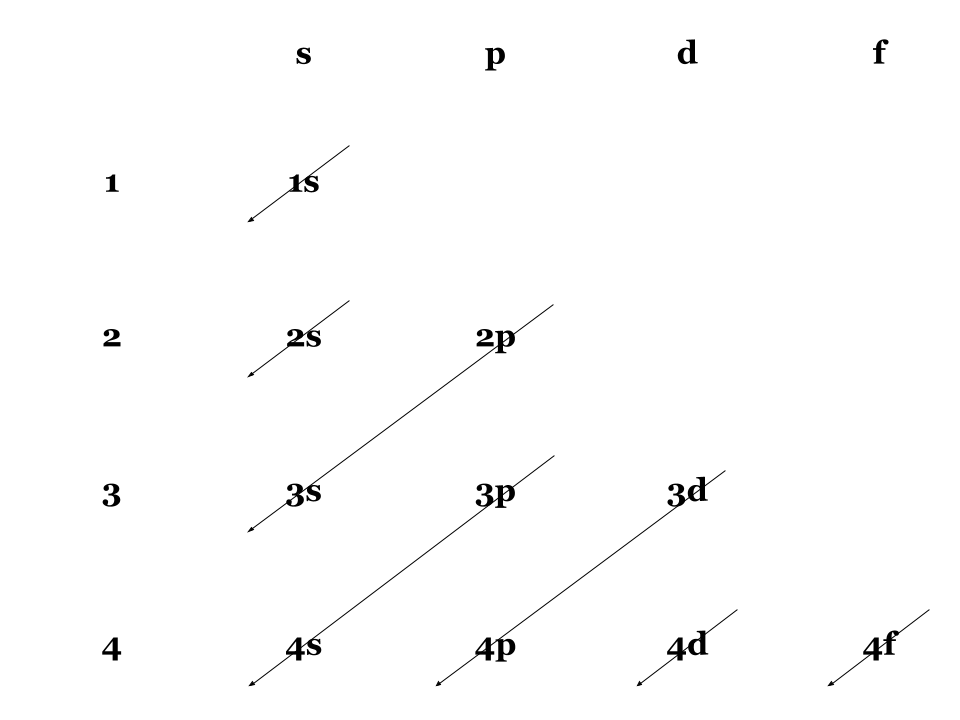
\includegraphics[width = .50\textwidth]{Electron_Config.png}\centering
\end{figure}
 \noindent The $s$ orbital can hold 2 electrons, $p$ can hold 6, $d$ can hold 10, and $f$ can hold 14. Therefore, the ground state electron configuration for phosphorus is

 \begin{gather}
 \boxed{1s^{2} 2s^{2} 2p^{6} 3s^{2} 3d^{3}}\nonumber
 \end{gather}
 \\
 Notice that, for larger electron numbers, $4s$ comes before $3d$.
\\\\
Answer: \textbf{\textcolor{ProcessBlue}B}\\

%%%%%%%%%%%%%%%%%%%%      18      %%%%%%%%%%%%%%%%%%%%

\section{\textsc{Problem 18:}} The key to this problem is to picture this system as a hydrogen-like atom (one electron) with two protons ($Z = 2$). The ionization energy of a hydrogen-like atom can be found using the equation

\begin{gather}
E_{n} = \frac{Z^{2}}{n^{2}} \unit[13.6]{[eV]}
\end{gather}
\\
where $n$ is the state of the system.

\begin{gather}
\therefore \hspace{.1in} E_{1} = Z^{2} \cdot \unit[13.6]{[eV]} = \unit[54.4]{[eV]}\nonumber
\end{gather}
\\
The problem tells us that the energy to remove both electrons from the He atom is $\unit[79.0]{[eV]}$. Therefore the energy required to remove one electron is

\begin{gather}
E_{ion} =  \unit[79.0]{[eV]} - \unit[54.4]{[eV]} = \boxed{\unit[24.6]{[eV]}}\nonumber
\end{gather}
\\\\
Answer: \textbf{\textcolor{ProcessBlue}A}\\

%%%%%%%%%%%%%%%%%%%%      19      %%%%%%%%%%%%%%%%%%%%

\section{\textsc{Problem 19:}} The primary source of the Sun's energy is the Proton-Proton Chain (PP Chain). in this reaction, \textbf{four H\textsuperscript{1}} atoms are fused an eventually create \textbf{one He\textsuperscript{4}} (I say "eventually" because there are 3 reactions in the PP Chain). From the mass-energy equivalence equation and conservation of energy, we know that the energy released during the PP Chain must be the difference in mass between four hydrogen atoms and one helium atom.
\\\\
Answer: \textbf{\textcolor{ProcessBlue}B}\\

%%%%%%%%%%%%%%%%%%%%      20      %%%%%%%%%%%%%%%%%%%%

\section{\textsc{Problem 20:}} This is pure fact recall. Bremsstrahlung refers to the electromagnetic radiation produced by the acceleration or deceleration of a charged particle (usually electrons) after passing through the electric and magnetic fields of a nucleus. This is a smooth, continuous X-ray spectra.
\\\\
Answer: \textbf{\textcolor{ProcessBlue}E}\\

%%%%%%%%%%%%%%%%%%%%      21      %%%%%%%%%%%%%%%%%%%%

\section{\textsc{Problem 21:}} The Rydberg formula for hydrogen is

\begin{gather}
f = \frac{c}{\lambda} = R \left(  \frac{1}{n_{f}^{2}} - \frac{1}{n_{i}^{2}}  \right)
\end{gather}
\\
Where $R$ is The Rydberg Constant and completely unnecessary for the purposes of this problem. Let us say that $\lambda '$ is the wavelength for Lyman-$\alpha$ and $\lambda$ is the wavelength for Balmer-$\alpha$

\begin{align}
\frac{\lambda' }{\lambda} &=  \frac{\left(  \frac{1}{n_{f}^{2}} - \frac{1}{n_{i}^{2}}  \right)}{\left(  \frac{1}{n_{f}'^{2}} - \frac{1}{n_{i}'^{2}}  \right)} = \frac{\left(   \frac{1}{4} - \frac{1}{9}   \right)   }{\left(    \frac{1}{1} -\frac{1}{4}   \right)} = \frac{\left(   \frac{9}{36} - \frac{4}{36}   \right)   }{\left(   \frac{3}{4}   \right)} = \frac{\frac{5}{36}}{\frac{3}{4}} = \frac{20}{108} = \boxed{\frac{5}{27}} \nonumber
\end{align}
\\
Make sure that you dont invert your fraction! Solution (E) is incorrect because it is Balmer-$\alpha$ to Lyman-$\alpha$ radiation and an excellent example of a common GRE a trap answer.
\\\\
Answer: \textbf{\textcolor{ProcessBlue}B}\\

%%%%%%%%%%%%%%%%%%%%      22      %%%%%%%%%%%%%%%%%%%%

\section{\textsc{Problem 22:}} The angular momentum of the moon is the same at every point in it's orbit. The equation for angular momentum, $L$, is

\begin{gather}
L = r \times p = m (r \times v) = m r v \sin{(\theta)}
\end{gather}
\\
The minimum, $r_{p}$, and maximum, $r_{a}$, distances (perigee and apogee) of the orbit correspond to a tangential velocity for which $\theta \hspace{.02in} = \hspace{.03in} 90^{^\circ}$.

\begin{gather}
L = m \cdot v_{a} \cdot r_{a} = m \cdot v_{p} \cdot r_{p}\
\end{gather}
\\
Obviously, we can cancel out the moon's mass, $m$, in the above conservation equation. Therefore we are unable to solve for this mass.\\
\\
Interesting tidbit: when the Soviet Union launched sputnik in 1957, American scientists were unable to determine the satellite's mass for this very reason.
\\\\
Answer: \textbf{\textcolor{ProcessBlue}A}\\

%%%%%%%%%%%%%%%%%%%%      23      %%%%%%%%%%%%%%%%%%%%

\section{\textsc{Problem 23:}} The particle is moving with a tangential velocity $v_{\perp} = \unitfrac[10]{[m]}{[s]}$ and the acceleration is $a_{rad} = \unitfrac[10]{[m]}{[s^{2}]}$. Since these values have the same magnitude, the angle between the velocity and acceleration vectors is $45^{\circ}$ (picture this as a 45-45-90 triangle).
\\\\
Answer: \textbf{\textcolor{ProcessBlue}C}\\

%%%%%%%%%%%%%%%%%%%%      24      %%%%%%%%%%%%%%%%%%%%

\section{\textsc{Problem 24:}} Gravity only applies in the vertical, $\hat{y}$, direction. Therefore $v_{x}$ is constant with respect to time. This eliminates (A) and (E).\\
\\
Since gravity is working in the $-\hat{y}$ direction while the stone is moving (partly) in the $+\hat{y}$ direction: $v_{y}$ starts positive and decreases with time. At the top of the stone's projectile motion $v_{y} = 0$. Then the stone begins to fall back to the ground so that $v_{y}$ is negative.
\\\\
Answer: \textbf{\textcolor{ProcessBlue}C}\\

%%%%%%%%%%%%%%%%%%%%      25      %%%%%%%%%%%%%%%%%%%%

\section{\textsc{Problem 25:}} The parallel axis theorem is an invaluable tool for computing the moment of inertia of systems built out of smaller pieces whose moments of inertia are known. The moment of inertia about any axis parallel to the center of mass axis is given by the equation

\begin{gather}
\label{eq:par_ax}I = I_{CM} +m r^{2}
\end{gather}
\\
One of these pennies (the middle one) has the same moment of inertia as a disk with radius $r$ and mass $m$. The other 6 require the the parallel axis theorem since the axis of rotation is $2r$ away from each penny's center of mass. The moment of inertia for a disk is $I = \frac{1}{2} m r^{2}$.

\begin{align}
I &= \frac{1}{2} m r^{2} + 6 \left(  \frac{1}{2}mr^2 + m (2r)^{2}  \right) = \frac{1}{2}mr^{2} + 6m r^{2} \left(  \frac{1}{2}  + \frac{8}{2}  \right)  = \boxed{\frac{55}{2} m r^{2}} \nonumber
\end{align}
\\\\
Answer: \textbf{\textcolor{ProcessBlue}E}\\

%%%%%%%%%%%%%%%%%%%%      26      %%%%%%%%%%%%%%%%%%%%

\section{\textsc{Problem 26:}} The moment of inertia for a rod is

\begin{gather}
I = \frac{1}{12} M L^{2}
\end{gather}
\\
We must use the parallel axis theorem (equation \ref{eq:par_ax}) again to to find the moment of inertia about the pivot:

\begin{gather}
I = \frac{1}{12} M L^{2} + M \left(   \frac{L}{2}  \right)^{2} = ML^{2} \left(  \frac{1}{12}  + \frac{3}{12}  \right) = \frac{1}{3}M L^{2}\nonumber
\end{gather}
\\
Now we need to find the speed of the pendulum once the free end hits the ground. The best and easiest way to do this is through use of conservation laws. The free end is $\frac{L}{2}$ above the rod's center of mass and $\omega = \frac{v}{L}$

\begin{align}
m g h &= \frac{1}{2} I \omega^{2}  \nonumber\\
M g \frac{L}{2} &= \frac{1}{2} \left(  \frac{1}{3} M L^{2}  \right) \frac{v^{2}}{L^{2}}   \nonumber\\
gL &= \frac{1}{3}v^{2} \hspace{.1in} \rightarrow \hspace{.1in} \boxed{v = \sqrt{3gL}}  \nonumber
\end{align}
\\\\
Answer: \textbf{\textcolor{ProcessBlue}C}\\

%%%%%%%%%%%%%%%%%%%%      27      %%%%%%%%%%%%%%%%%%%%

\section{\textsc{Problem 27:}} The eigenvalues of a Hermitian operator are always real.\\
\\
Proof: The eigenvalue equation is

\begin{align}
A \ket{\psi} &= \lambda \ket{\psi}\nonumber\\
\therefore \hspace{.1in} A^{\dag} \ket{\psi} &= \lambda^{*} \ket{\psi}\nonumber
\end{align}
\\
Subtracting the second equation from the first we get

\begin{gather}
( A - A^{\dag} )\ket{\psi} = ( \lambda - \lambda^{*} ) \ket{\psi}\nonumber
\end{gather}
The left hand side of the above equation is equal to zero since $A = A^{\dag}$. Therefore, $\lambda = \lambda^{*}$ which means that $\lambda$ is real-valued.
\\\\
Answer: \textbf{\textcolor{ProcessBlue}A}\\

%%%%%%%%%%%%%%%%%%%%      28      %%%%%%%%%%%%%%%%%%%%

\section{\textsc{Problem 28:}} Lets say that states n and m are orthonormal: $\braket{ n  | m } = 0$ and $\braket{ n  | n } = \braket{ m  | m } = 1$. Therefore:

\begin{align}
\braket{\psi_{1} | \psi_{2}} &= 0\nonumber\\
&= 5 \braket{ 1 | 1 }  + 15 \braket{ 2 | 2 }  + 2x \braket{ 3 | 3 } \nonumber\\
0 &= 20 + 2x \hspace{.1in} \rightarrow \hspace{.1in} \boxed{x = - 10}\nonumber
\end{align}
\\\\
Answer: \textbf{\textcolor{ProcessBlue}E}\\

%%%%%%%%%%%%%%%%%%%%      29      %%%%%%%%%%%%%%%%%%%%

\section{\textsc{Problem 29:}} Recall the Dirac notation identity:

\begin{gather}
\bra{\psi} \hat{A} \ket{\psi} =  \lambda \braket {\psi  | \psi} = \lambda
\end{gather}
\\
Where $\lambda$ is an eigenvalue of $\hat{A}$. From this we can see that, using our given eigenvalues, we get

\begin{align}
\bra{\psi_{-1}} \hat{0} \ket{\psi_{-1}} &= -1 \braket {\psi_{-1}  | \psi_{-1}} = -1\nonumber\\
\bra{\psi_{1}} \hat{0} \ket{\psi_{1}} &= 1 \braket {\psi_{1}  | \psi_{1}} = 1\nonumber\\
\bra{\psi_{2}} \hat{0} \ket{\psi_{2}} &= 2 \braket {\psi_{2}  | \psi_{2}} = 2\nonumber
\end{align}
\\
Therefore,

\begin{gather}
\bra{\psi} \hat{O} \ket{\psi} = \frac{1}{6} \braket {\psi_{-1}  | \psi_{-1}} + \frac{1}{2} \braket {\psi_{1}  | \psi_{1}} + \frac{1}{3} \braket {\psi_{2}  | \psi_{2}} = -\frac{1}{6} + \frac{1}{2} + \frac{2}{3} = \boxed{1}\nonumber
\end{gather}
\\\\
Answer: \textbf{\textcolor{ProcessBlue}C}\\

%%%%%%%%%%%%%%%%%%%%      30      %%%%%%%%%%%%%%%%%%%%

\section{\textsc{Problem 30:}} This kind of problem begs for the process of elimination. Radial wave functions must be normalizable and must go to zero at infinity. Therefore:

\begin{description}
\item[I.] Works. it is normalizable (square integrable) and goes to zero at infinity.

\item[II.] Doesn't work. Sinusoidal functions do not converge and therefore do not go to zero at infinity.

\item[III.] Doesn't work. This function is not normalizable.
\end{description}
Answer: \textbf{\textcolor{ProcessBlue}A}\\

%%%%%%%%%%%%%%%%%%%%      31      %%%%%%%%%%%%%%%%%%%%

\section{\textsc{Problem 31:}} The ground state energy of hydrogen is

\begin{gather}
E_{0,H} = \unit[13.6]{[eV]} \propto \mu
\end{gather}
\\
where $\mu$ is the reduced mass of the system given by the equation

\begin{gather}
\mu = \frac{m_{1} \cdot m_{2}}{m_{1} + m_{2}}
\end{gather}
\\
For a normal hydrogen atom, $\mu \approx m_{e}$ (because $m_{p} \gg m_{e}$). For positronium:

\begin{gather}
\mu = \frac{m_{e} \cdot m_{e}}{m_{e} + m_{e}} = \frac{me}{2}\nonumber
\end{gather}
\\
or 1/2 the reduced mass of hydrogen. Therefore the ground state energy of positronium is

\begin{gather}
E_{0,p} = \frac{\unit[13.6]{[eV]}}{2} = \unit[6.8]{[eV]}\nonumber
\end{gather}
\\
Now, we are looking for the energy of the photon emitted when the positronium makes the transition from $n = 3$ to $n = 1$:

\begin{gather}
E_{\gamma} = \unit[6.8]{[eV]} \cdot \left(  \frac{1}{n^{2}_{f}} - \frac{1}{n^{2}_{i}} \right) = \unit[6.8]{[eV]}  \cdot \left(  \frac{9}{9} - \frac{1}{9} \right) = \unit[6.8]{[eV]}  \cdot \left(  \frac{8}{9}   \right) = \frac{\unit[54]{[eV]} }{9} = \boxed{\unit[6]{[eV]}} \nonumber
\end{gather}
\\\\
Answer: \textbf{\textcolor{ProcessBlue}A}\\

%%%%%%%%%%%%%%%%%%%%      32      %%%%%%%%%%%%%%%%%%%%

\section{\textsc{Problem 32:}} The relativistic energy-momentum relation is

\begin{gather}
\label{eq:rel-energy} E^{2} = (pc)^{2} + (m_{0} c^{2})^{2}
\end{gather}
\\
The given particle has $m_{0} = m$ and $E = 2mc^{2}$. Solving for $p$ in the above equation

\begin{gather}
p^{2} = \frac{E^{2}}{c^{2}} -  m_{0}^{2}c^{2}  =  \frac{(2mc^{2})^{2}}{c^{2}} -  m^{2}c^{2}  = \frac{4m^{2}c^{4}}{c^{2}} -  m^{2}c^{2} = 3m^{2}c^{2}\nonumber\\
\nonumber\\
\therefore \hspace{.1in} p = \sqrt{3m^{2}c^{2}} = \boxed{\sqrt{3} m c}\nonumber
\end{gather}
\\\\
Answer: \textbf{\textcolor{ProcessBlue}D}\\

%%%%%%%%%%%%%%%%%%%%      33      %%%%%%%%%%%%%%%%%%%%

\section{\textsc{Problem 33:}} Let us say that the particle's rest frame is $S'$ and the lab frame is $S$. The Lorentz Invariance Formula is:

\begin{gather}
\left(  \Delta x  \right)^{2}  - \left(  c \Delta t  \right)^{2}  = \left(  \Delta x'  \right)^{2}  - \left(  c \Delta t'  \right)^{2}
\end{gather}
\\
We are given that $\Delta t' = \unit[10^{-8}]{[s]}$, $\Delta x = \unit[30]{[m]}$, and $\Delta x' = \unit[0]{[m]}$ (since $S'$ is the particle's rest frame). So let us solve for $\Delta t$:

\begin{gather}
\Delta t = \sqrt{\frac{\Delta x^{2}}{c^{2}} + \Delta t'^{2}}\nonumber
\end{gather}
\\
we are solving for the speed of the pion which can be found using the equation

\begin{align}
v &= \frac{\Delta x}{\Delta t}\\
&= \Delta x \left(   \frac{\Delta x^{2}}{c^{2}} + \Delta t'^{2}   \right)^{-\frac{1}{2}} = c \Delta x \left(   \Delta x^{2} + c^{2}\Delta t'^{2}   \right)^{-\frac{1}{2}}\nonumber\\
\nonumber\\
&= \frac{c \cdot \unit[30]{[m]}}{\sqrt{\unit[900]{[m^{2}]} + (\unitfrac[3\e{8}]{[m]}{[s]})^{2} \cdot (\unit[10^{-16}]{[s^{2}]})}} = c \cdot\sqrt{    \frac{\unit[900]{[m^{2}]}}{\unit[900]{[m^{2}]} + \unit[9]{[m^{2}]} }     }\nonumber\\
\nonumber\\
 &= c \cdot \sqrt{\frac{100}{101}} \approx \boxed{\unitfrac[2.98]{[m]}{[s]}}\nonumber
\end{align}
\\\\
Answer: \textbf{\textcolor{ProcessBlue}D}\\

%%%%%%%%%%%%%%%%%%%%      34      %%%%%%%%%%%%%%%%%%%%

\section{\textsc{Problem 34:}} In special relativity there are three different classifications of invariant intervals:

\begin{description}
\item[I.] \textbf{Space-like}: $\Delta s^{2} > 0$.  These events can occur simultaneously for some observers but are separated in space.

\item[II.] \textbf{Time-like}: $\Delta s^{2} < 0$. These events can occur at the same location but are separated by time.

\item[III.] \textbf{Light-like}: $\Delta s^{2} = 0$. Only something traveling at the speed of light could be present at both events.
\end{description}
In this problem we are being asked about when the interval is \textbf{Space-like}.

\begin{align}
 0 < \Delta s^{2}   =  \Delta x^{2} - c^{2} \Delta t^{2} \hspace{.1in} \rightarrow \hspace{.1in}
 \Delta x^{2} <  c^{2} \Delta t^{2} \hspace{.1in} \rightarrow \hspace{.1in}
 \boxed{\left|   \frac{\Delta x}{\Delta t} \right| < c}\nonumber
\end{align}
\\\\
Answer: \textbf{\textcolor{ProcessBlue}B}\\

%%%%%%%%%%%%%%%%%%%%      35      %%%%%%%%%%%%%%%%%%%%

\section{\textsc{Problem 35:}} The Stefan-Boltzmann Law is

\begin{gather}
dP = \epsilon \sigma T^{4} dA \hspace{.1in} \rightarrow \hspace{.1in} \frac{dP}{dA} \propto T^{4}
\end{gather}
\\
Therefore, if the temperature increases by a factor of 3, the energy radiated per second per unit area is

\begin{gather}
\frac{dP}{dA} \propto \boxed{3^{4} = 81}\nonumber
\end{gather}
\\\\
Answer: \textbf{\textcolor{ProcessBlue}E}\\

%%%%%%%%%%%%%%%%%%%%      36      %%%%%%%%%%%%%%%%%%%%

\section{\textsc{Problem 36:}} Process of elimination:

\begin{description}

\item[(A)] True. This is the definition of an adiabatic process.

\item[(B)] True. There is no change in entropy in a quasi-static expansion.

\item[(C)] True.  $\Delta U = \Delta Q - \Delta W$ while $\Delta Q=0$ for an adiabatic process and $\Delta W = \int P dV$. Therefore, $\Delta U =  -\int P dV$

\item[(D)] True. See above.

\item[(E)] False. $\Delta W = P \Delta V = N k  \Delta T$. Do not confuse adiabatic ($\Delta Q = 0$) and isothermal  ($\Delta T = 0$) processes. \\

\end{description}
Answer: \textbf{\textcolor{ProcessBlue}E}\\

%%%%%%%%%%%%%%%%%%%%      37      %%%%%%%%%%%%%%%%%%%%

\section{\textsc{Problem 37:}} The area inside a closed loop on a PV diagram is the work done by the process. The direction of the cycle determines the sign of the work (convention: clockwise is positive, counterclockwise is negative). From this information we can eliminate (A), (B), and (C).\\
\\
we can determine the volume at $B$, $V_{B}$, using the ideal gas law $P V = n R T$. Because $BC$ is an isothermal (constant temperature) process

\begin{gather}
P_{B} V_{B} = const = P_{C} V_{C} \hspace{.1in} \rightarrow \hspace{.1in} V_{B} = \frac{P_{C} V_{C}}{P_{B}} = \frac{\unit[500]{[kPa]} \cdot \unit[2]{[m^{3}]}}{\unit[200]{[kPa]}} = \unit[5]{[m^{3}]}\nonumber
\end{gather}
\\
Now, let us approximate the cycle as a right triangle with height $P = \unit[500]{[kPa]}-\unit[200]{[kPa]} = \unit[500]{[kPa]}$ and base $V = \unit[5]{[m^{3}]} - \unit[2]{[m^{3}]} = \unit[3]{[m^{3}]}$. The area of this triangle (read: magnitude of work done) would be

\begin{gather}
A = |W| = \frac{1}{2} (\unit[3]{[m^{3}]}) (\unit[500]{[kPa]}) = \unit[450]{[kJ]}
\end{gather}
\\
Because the area of the actual process is less than the area of our approximated triangle we can eliminate (E).
\\\\
Answer: \textbf{\textcolor{ProcessBlue}D}\\

%%%%%%%%%%%%%%%%%%%%      38      %%%%%%%%%%%%%%%%%%%%

\section{\textsc{Problem 38:}} The current is maximized when the resonant frequency is reached. The resonant frequency is reached when the complex impedance is 0:

\begin{gather}
X_{C} - X_{L} = \frac{1}{\omega C} - \omega L = 0 \hspace{.1in} \rightarrow \hspace{.1in} \frac{1}{\omega C} = \omega L \hspace{.1in} \rightarrow \hspace{.1in} \omega = \frac{1}{\sqrt{LC}}
\end{gather}
\\
Solving for $C$ and plugging in the given values for $\omega$ and $L$ we get

\begin{gather}
C = \frac{1}{L \omega^{2}} =  \frac{1}{\unit[25]{[mH]} (\unitfrac[1000]{[rads]}{[s]})^{2}}  = \unit[4\e{-5}]{[F]} = \boxed{\unit[40]{[\mu F]}} \nonumber
\end{gather}
\\\\
Answer: \textbf{\textcolor{ProcessBlue}D}\\

%%%%%%%%%%%%%%%%%%%%      39      %%%%%%%%%%%%%%%%%%%%

\section{\textsc{Problem 39:}} A high-pass filter is a series combination of a \textbf{Capacitor followed by a Resistor} or a \textbf{Resistor followed by an Inductor} (CR or RL)\\
\\
The inverse is a low-pass filter: a  series combination of a \textbf{Resistor followed by a Capacitor} or an \textbf{Inductor followed by a Resistor} (RC or LR)
\\\\
Answer: \textbf{\textcolor{ProcessBlue}D}\\

%%%%%%%%%%%%%%%%%%%%      40      %%%%%%%%%%%%%%%%%%%%

\section{\textsc{Problem 40:}} We can eliminate (B), (C) and (E) based on the fact that the time constant of the ciruit is

\begin{gather}
\tau = \frac{L}{R} = \frac{\unit[10\e{-3}]{[H]}}{\unit[2]{[\Omega]}} = \unit[5\e{-3}]{[s]} = \unit[5]{[ms]}
\end{gather}
\\
The voltage with with respect to time can be calculated using the equation

\begin{gather}
V(t) = V_{0} e^{-t/\tau}
\end{gather}
\\
So that at $t=0$ the voltage is $\unit[10]{[V]}$
\\\\
Answer: \textbf{\textcolor{ProcessBlue}D}\\

%%%%%%%%%%%%%%%%%%%%      41      %%%%%%%%%%%%%%%%%%%%

\section{\textsc{Problem 41:}} Gauss's law for magnetism $\nabla \cdot \vec{B} = 0$ is the mathematic statement "Magnetic monopoles do not exist." Therefore, we can eliminate (A), (C), and (D) since they do not include II.\\
\\
If magnetic monopoles were to exist, Maxwell's Equations would be symmetric with their counterparts (divergence and curl). Therefore, we would have to change both II (as discussed above) and IV.
\\\\
Answer: \textbf{\textcolor{ProcessBlue}E}\\

%%%%%%%%%%%%%%%%%%%%      42      %%%%%%%%%%%%%%%%%%%%

\section{\textsc{Problem 42:}} The induced current in loops $A$ and $B$ follows the equation

\begin{gather}
\mathcal{E} = -\frac{d \Phi_{B}}{d t} = -A \frac{d B}{dt}
\end{gather}
\\
The minus sign in this equation is a statement that the current inducted opposes the changing field. Therefore as the current loop moves towards $A$ the magnetic field increases at $A$ and the induced current is clockwise. at the same time, the magnetic field decreases at $B$ and the induced current is counterclockwise.
\\\\
Answer: \textbf{\textcolor{ProcessBlue}C}\\

%%%%%%%%%%%%%%%%%%%%      43      %%%%%%%%%%%%%%%%%%%%

\section{\textsc{Problem 43:}} \textbf{Memorize this identity}:

\begin{gather}
[AB, C] = B [A, C] + [B, C] A
\end{gather}
\\
Using this, the given commutator comes out to

\begin{align}
[L_{x}L_{y}, L_{z}] &= L_{y} [L_{x}, L_{z}] + [L_{y}, L_{z}] L_{x}\nonumber\\
&= L_{y} (-i \hbar L_{y}) + (i \hbar L_{x})L_{x} = i \hbar ( L_{x}^{2} -  L_{y}^{2} )\nonumber
\end{align}
\\\\
Answer: \textbf{\textcolor{ProcessBlue}D}\\

%%%%%%%%%%%%%%%%%%%%      44      %%%%%%%%%%%%%%%%%%%%

\section{\textsc{Problem 44:}} Everything that you need is given to you in the problem statement. If

\begin{gather}
E_n = \frac{n^{2} \pi^{2} \hbar^{2}}{2mL^{2}}
\end{gather}
\
then
\begin{align}
E_1 &= \frac{\pi^{2} \hbar^{2}}{2mL^{2}}\nonumber\\
\nonumber\\
E_2 &= \frac{4 \pi^{2} \hbar^{2}}{2mL^{2}} = 4E_{1}\nonumber\\
\nonumber\\
E_3 &= \frac{9 \pi^{2} \hbar^{2}}{2mL^{2}} = \boxed{9E_{1}}\nonumber
\end{align}
\\\\
Answer: \textbf{\textcolor{ProcessBlue}D}\\

%%%%%%%%%%%%%%%%%%%%      45      %%%%%%%%%%%%%%%%%%%%

\section{\textsc{Problem 45:}} First, solve for the $H \ket{n}$ from $n = 1$ to $n = 3$:

\begin{align}
H \ket{1} &= \frac{3}{2} \hbar \omega  \ket{1}\nonumber\\
\nonumber\\
H \ket{2} &= \frac{5}{2} \hbar \omega  \ket{2}\nonumber\\
\nonumber\\
H \ket{3} &= \frac{7}{2} \hbar \omega  \ket{3}\nonumber
\end{align}
\\
The inner product is therefore,

\begin{align}
\bra{\psi}H \ket{\psi} &= \frac{1}{14} \left(   \frac{3}{2} \hbar \omega\right)  + \frac{4}{14} \left(   \frac{5}{2} \hbar \omega\right) +  \frac{9}{14} \left(   \frac{7}{2} \hbar \omega \right) \nonumber\\
\nonumber\\
&= \left(   \frac{3}{28}  + \frac{20}{28}  + \frac{63}{28} \right) \hbar \omega = \frac{86}{28} \hbar \omega = \boxed{\frac{43}{14} \hbar \omega}   \nonumber
\end{align}
\\\\
Answer: \textbf{\textcolor{ProcessBlue}B}\\

%%%%%%%%%%%%%%%%%%%%      46      %%%%%%%%%%%%%%%%%%%%

\section{\textsc{Problem 46:}} The two equations that you need for this problem are the de Broglie formula and the kinetic energy equation:

\begin{gather}
\lambda = \frac{h}{p} \hspace{.1in} \\
T = \frac{1}{2}mv^{2} = \frac{p^{2}}{2m}
\end{gather}
\\
Noting that $h$ is a constant, we can rewrite the de Broglie formula:

\begin{gather}
\lambda_{0} p_{0} = h = \lambda_{f} p_{f} \hspace{.1in} \rightarrow \hspace{.1in} \lambda_{f} = \frac{\lambda_{0} p_{0}}{p_{f}} \nonumber
\end{gather}
\\
Then we can rewrite the kinetic energy equations:

\begin{gather}
T_{0} = E = \frac{p_{0}^{2}}{2m} \hspace{.1in} \rightarrow \hspace{.1in} p_{0} = \sqrt{2mE}\nonumber\\
T_{f} = E-V = \frac{p_{f}^{2}}{2m} \hspace{.1in} \rightarrow \hspace{.1in} p_{f} = \sqrt{2m(E-V)}\nonumber
\end{gather}
\\
Therefore,

\begin{gather}
\lambda_{1} = \frac{\lambda_{0} \sqrt{2mE}}{\sqrt{2m(E-V)}} = \lambda_{0}\sqrt{\frac{E}{E-V}} = \lambda_{0}\sqrt{\frac{1}{1-V/E}} = \boxed{\lambda_{0} \left(  1- V/E \right)^{-1/2}}\nonumber
\end{gather}
\\\\
Answer: \textbf{\textcolor{ProcessBlue}E}\\

%%%%%%%%%%%%%%%%%%%%      47      %%%%%%%%%%%%%%%%%%%%

\section{\textsc{Problem 47:}} From the second law of thermodynamics we know that

\begin{gather}
\Delta S = \int{\frac{dQ}{T}} = \frac{1}{T} \int{dQ}
\end{gather}
\\
because this container is sealed and thermally insulated $\Delta U = 0$. Therefore, from the first law of thermodynamics,   $d Q=dW$.

\begin{gather}
\Delta S = \int{\frac{dQ}{T}} = \frac{1}{T} \int{dW} = \frac{1}{T} \int{P dV} = nR \int{\frac{ dV}{V}}_{1}^{2} = nR\ln{(2/1)} = \boxed{n R \ln{(2)}}\nonumber
\end{gather}
\\\\
Answer: \textbf{\textcolor{ProcessBlue}B}\\

%%%%%%%%%%%%%%%%%%%%      48      %%%%%%%%%%%%%%%%%%%%

\section{\textsc{Problem 48:}} The rms velocity equation can be found by equating the kinetic energy of a gas particle to the total kinetic energy of the gas:

\begin{gather}
\frac{1}{2}mv^{2} = \frac{3}{2} k T \hspace{.1in} \rightarrow \hspace{.1in} v_{rms} = \sqrt{\frac{3kT}{m}}
\end{gather}
\\
Therefore with constant temperature, the ratio of $v_{rms}(N_{2})$ to $v_{rms}(O_{2})$ is

\begin{gather}
\frac{v_{rms}(N_{2})}{v_{rms}(O_{2})} = \frac{\sqrt{m_{O_{2}}}}{\sqrt{m_{N_{2}}}} = \frac{\sqrt{32}}{\sqrt{28}} = \boxed{\sqrt{\frac{8}{7}}}\nonumber
\end{gather}
\\\\
Answer: \textbf{\textcolor{ProcessBlue}C}\\

%%%%%%%%%%%%%%%%%%%%      49      %%%%%%%%%%%%%%%%%%%%

\section{\textsc{Problem 49:}} The partition function, $Z$, of a non-degenerate system is

\begin{gather}
Z = \sum_{n}{e^{-E_{n}/kT}} = e^{-\epsilon/kT} + e^{-2 \epsilon/kT}
\end{gather}
\\
Taking into account the degeneracy, $d$, of the system: the degenerate partition function, $Z_{D}$, is

\begin{gather}
Z_{D} = \sum_{n}{d_{n} e^{-E_{n}/kT}} =2 \left( e^{-\epsilon/kT} + e^{-2 \epsilon/kT}  \right)
\end{gather}
\\\\
Answer: \textbf{\textcolor{ProcessBlue}E}\\

%%%%%%%%%%%%%%%%%%%%      50      %%%%%%%%%%%%%%%%%%%%

\section{\textsc{Problem 50:}} From Wien's Law we know that $\lambda_{} T_{}  = const$. The wavelength is related to frequency by the equation  $\lambda_{} = c/\nu_{}$. Therefore

\begin{gather}
T_{1}  \frac{c_{1}}{\nu_{1}} = const = T_{2}  \frac{c_{2}}{\nu_{2}}\nonumber
\end{gather}
\\
From the problem, we know that $T_{1} = T_{2}$, $\nu_{1} = \unit[440]{[Hz]}$, and $c_{2}  = 0.97 \cdot c_{1}$. Plugging in:

\begin{gather}
\frac{c_{1}}{\nu_{1}} = \frac{0.97 c_{1}}{\nu_{2}} \hspace{.1in} \rightarrow \hspace{.1in} \nu_{2} = 0.97 \cdot \nu_{1} = 0.97 \cdot \unit[440]{[Hz]} \approx \boxed{\unit[427]{[Hz]}}\nonumber
\end{gather}
\\\\
Answer: \textbf{\textcolor{ProcessBlue}B}\\

%%%%%%%%%%%%%%%%%%%%      51      %%%%%%%%%%%%%%%%%%%%

\section{\textsc{Problem 51:}} The intensity light through the first polarizer, $I_{1}$, is half the the intensity of the initial beam:

\begin{gather}
I_{1} = \frac{I_{0}}{2}
\end{gather}
\\
Now, we must use Malus' Law, $I_{f} = I_{i} \cos^{2}{\theta}$ where $\theta = 45^{\circ}$ for the second polarizer and then $\theta = 45^{\circ}$ again for the third and final polarizer.

\begin{gather}
I_{2} = I_{1} \cos^{2}{45^{\circ}} = \frac{I_{1}}{2} = \frac{I_{0}}{4}\nonumber\\
I_{3} = I_{2} \cos^{2}{45^{\circ}} = \frac{I_{2}}{2} = \boxed{\frac{I_{0}}{8}}\nonumber
\end{gather}
\\\\
Answer: \textbf{\textcolor{ProcessBlue}B}\\

%%%%%%%%%%%%%%%%%%%%      52      %%%%%%%%%%%%%%%%%%%%

\section{\textsc{Problem 52:}} The volume of the primitive unit cell is the the volume of conventional unit cell divided by the number of lattice points in the Bravais lattice. A body-centered cubic lattice (BCC) has two lattice points (only count the sections inside the lattice) so that the volume is $\boxed{a^{3}/2}$\\
\\
In case you were wondering: A Bravais lattice is one that is isotropic at every point. A face centered cubic lattice (FCC) has four lattice points and a simple cubic lattice has one lattice point.
\\\\
Answer: \textbf{\textcolor{ProcessBlue}B}\\

%%%%%%%%%%%%%%%%%%%%      53      %%%%%%%%%%%%%%%%%%%%

\section{\textsc{Problem 53:}} Recall the resistivity equation from elementary electrodynamics:

\begin{gather}
R = R_{0}  \left( 1 + \alpha \Delta T  \right) \hspace{.1in} \rightarrow \hspace{.1in} \rho = \rho_{0}  \left( 1 + \alpha \Delta T  \right)
\end{gather}
\\
semiconductors have a negative coefficient of resistivity, $\alpha$, which means that the resistivity, $\rho$, should should decrease with increasing temperature. (B) choice
\\\\
Answer: \textbf{\textcolor{ProcessBlue}B}\\

%%%%%%%%%%%%%%%%%%%%      54      %%%%%%%%%%%%%%%%%%%%

\section{\textsc{Problem 54:}} The total impulse, $j$, delivered to a particle can be found using the equation:

\begin{gather}
j = \int{F \cdot dt}
\end{gather}
\\
Which is just the area under the curve of a Force vs time plot. The area is easy to calculate since the function forms a triangle:

\begin{gather}
j = \frac{1}{2}(\unit[2]{[N]} \cdot \unit[2]{[s]}) = \boxed{\unitfrac[2]{[kg \cdot m]}{[s]}}\nonumber
\end{gather}
\\\\
Answer: \textbf{\textcolor{ProcessBlue}C}\\

%%%%%%%%%%%%%%%%%%%%      55      %%%%%%%%%%%%%%%%%%%%

\section{\textsc{Problem 55:}} This is a simple application of the momentum conservation laws.

\begin{align}
p_{i} &= p_{f}\nonumber\\
mv + (2m) (0) &= (m) (0) + m v' \cos{(\theta)} + m v' \cos{(\theta)} \nonumber\\
mv &=  2m v' \cos{(\theta)} \hspace{.1in} \rightarrow \hspace{.1in} v' = \frac{v}{2\cos{(\theta)}}\nonumber
\end{align}
\\
$\cos{(\theta)}$ is always between zero and one so that $v/2 \leq v < \infty$
\\\\
Answer: \textbf{\textcolor{ProcessBlue}E}\\

%%%%%%%%%%%%%%%%%%%%      56      %%%%%%%%%%%%%%%%%%%%

\section{\textsc{Problem 56:}} This is a force balancing problem in which we imagine the ballon is stationary, i.e. the upward force is equal to the downward force.

\begin{align}
  V g \rho_{air} &= mg + V g \rho_{He} \nonumber\\
  \nonumber\\
 V&= \frac{ m  }{ \rho_{air} - \rho_{He} }  =  \frac{ \unit[300]{[kg]}  }{ \unitfrac[1.29]{[kg]}{[m^{3}]} - \unitfrac[0.18]{[kg]}{[m^{3}]} } =  \boxed{\unit[270]{[m^{3}]} }\nonumber
\end{align}
\\\\
Answer: \textbf{\textcolor{ProcessBlue}D}\\

%%%%%%%%%%%%%%%%%%%%      57      %%%%%%%%%%%%%%%%%%%%

\section{\textsc{Problem 57:}} The momentum of the stream is

\begin{gather}
p = v dm= v \rho \cdot dV = v \rho \cdot A (dx) = v \rho \cdot A (v dt )\nonumber
\end{gather}
\\
We know from Newton's second law that $F =\dot{p}$ so that

\begin{gather}
F = \frac{d p}{d t} = \rho v^{2} A \frac{dt}{dt} =  \rho v^{2} A \nonumber
\end{gather}
\\\\
Answer: \textbf{\textcolor{ProcessBlue}A}\\

%%%%%%%%%%%%%%%%%%%%      58      %%%%%%%%%%%%%%%%%%%%

\section{\textsc{Problem 58:}} The Lorentz force equation is

\begin{gather}
\vec{F} = q (\vec{E} + \vec{v} \times \vec{B})
\end{gather}
\\
we can find the velocity, $v$ , of the proton by equating the particle's translational kinetic energy to its kinetic energy in a potential, $V \hat{z}$.

\begin{gather}
\frac{1}{2} m \vec{v}^{2} = q V \hat{z} \hspace{.1in} \rightarrow \hspace{.1in} \vec{v} = \sqrt{\frac{2qV}{m}}\hat{z}
\end{gather}
\\
The electric and magnetic fields are directed in the $+\hat{x}$ and $+\hat{y}$ direction, respectively, so that

\begin{align}
\vec{F} &= q (E\hat{x} + v\hat{z} \times B \hat{y}) \nonumber\\
&= q (E\hat{x} - vB\hat{x})
\end{align}
\\
When the particle's trajectory is not affected, $F = 0$ so that $E =vB$. However, if we are to increase the potential to $V' = 2V$ then

\begin{gather}
\vec{v'} = \sqrt{\frac{2qV'}{m}}\hat{z} = \sqrt{\frac{4qV}{m}}\hat{z} > \vec{v}
\end{gather}
\\
With this potential $E < vB$ and the resultant force is therefore the $\boxed{-\hat{x}}$ direction.
\\\\
Answer: \textbf{\textcolor{ProcessBlue}B}\\

%%%%%%%%%%%%%%%%%%%%      59      %%%%%%%%%%%%%%%%%%%%

\section{\textsc{Problem 59:}} The equation for simple harmonic motion of an oscillator is

\begin{gather}
m \frac{d^{2}x}{dt^{2}} + kx = 0
\end{gather}
\\
The analogous equation for the given circuit must have $\boxed{L = m\text{, }Q = x\text{, and }C = \frac{1}{k}}$
\\\\
Answer: \textbf{\textcolor{ProcessBlue}B}\\

%%%%%%%%%%%%%%%%%%%%      60      %%%%%%%%%%%%%%%%%%%%

\section{\textsc{Problem 60:}} The electric flux is

\begin{gather}
\Phi_{E} = \int{E \cdot dA} = \frac{Q}{\epsilon_{0}} = \frac{\sigma A}{\epsilon_{0}} = \frac{\sigma \pi c^{2}}{\epsilon_{0}}
\end{gather}
\\
where $c$ is the radius of the sheet's affected area and can be calculated via the pythagorean theorem:

\begin{gather}
R^{2} = c^{2} + x^{2} \hspace{.1in} \rightarrow \hspace{.1in} c^{2} = R^{2} - x^{2}\nonumber\\
\nonumber\\
\therefore \hspace{.1in} \boxed{\Phi_{E} = \frac{\sigma \pi \left(   R^{2} - x^{2}  \right)}{\epsilon_{0}}}\nonumber
\end{gather}
\\\\
Answer: \textbf{\textcolor{ProcessBlue}D}\\

%%%%%%%%%%%%%%%%%%%%      61      %%%%%%%%%%%%%%%%%%%%

\section{\textsc{Problem 61:}} When an electromagnetic wave comes into contact with a conductor $E = 0$ and $B \neq 0$. This is because electric fields don't propagate through conductors but they do cause the surface charges to move back and forth, which creates and oscillating magnetic field. The only solution that fits these conditions is (C).
\\\\
Answer: \textbf{\textcolor{ProcessBlue}C}\\

%%%%%%%%%%%%%%%%%%%%      62      %%%%%%%%%%%%%%%%%%%%

\section{\textsc{Problem 62:}} The cyclotron frequency follows the simple equation $f = \omega/2 \pi$ where

\begin{gather}
\omega = \frac{qB}{ m}\\
\nonumber\\
\therefore \hspace{.1in}  f = \frac{qB}{2 \pi m}  \hspace{.1in} \rightarrow \hspace{.1in} m = \frac{q B }{2 \pi f}   \nonumber
\end{gather}
\\
Plugging in the given values:

\begin{gather}
m = \frac{(2 e) (\unit[\pi / 4]{[T]}) }{2 \pi \cdot \unit[1,600]{[Hz]}} = \frac{  e  }{ \unit[1,600]{[Hz]}} \cdot \unit[\frac{1}{4}]{[T]} = \boxed{\unit[2.5\e{-23}]{[kg]}}\nonumber
\end{gather}
\\\\
Answer: \textbf{\textcolor{ProcessBlue}A}\\

%%%%%%%%%%%%%%%%%%%%      63      %%%%%%%%%%%%%%%%%%%%

\section{\textsc{Problem 63:}} Simple application of Wein's Law

\begin{gather}
T = \frac{\unit[2.9\e{-3}]{[m \cdot K]}}{\lambda} = \frac{\unit[2.9\e{-3}]{[m \cdot K]}}{\unit[2\e{-6}]{[m]}} \approx \frac{3}{2} \e{3} =\boxed{\unit[1,500]{K}}
\end{gather}
\\\\
Answer: \textbf{\textcolor{ProcessBlue}D}\\

%%%%%%%%%%%%%%%%%%%%      64      %%%%%%%%%%%%%%%%%%%%

\section{\textsc{Problem 64:}} Process of elimination:

\begin{description}
\item[(A)] Spectral lines are due to electrons changing energy levels. Therefore, the word "nuclear" makes this answer seam a little suspect. Lets check out the others.

\item[(B)] The wavelength associated in the absorption spectrum and usually very close to those of the emission spectrum. This is true.

 \item[(C)] Astrophysicists often use the absorption spectrum to determine the composition of stars. This is true.

 \item[(D)] See above. This is true.

 \item[(E)] A band spectrum is defined as a spectrum consisting of a number of closely spaced bands that are associated with emission or absorption of radiation by \textbf{molecules}. So yes, this is also true.
\end{description}
Answer: \textbf{\textcolor{ProcessBlue}A}\\

%%%%%%%%%%%%%%%%%%%%      65      %%%%%%%%%%%%%%%%%%%%

\section{\textsc{Problem 65:}} At high temperatures $h \nu/kT$  is a very small number. Therefore we can use the identity

\begin{gather}
e^{x} \approx 1+x
\end{gather}
\\
where $x = h \nu/kT$ so that the equation is can be written as

\begin{align}
C &= 3kN_{A} \left(  \frac{h\nu}{kT}  \right)^{2} \frac{e^{h\nu/kt}}{\left(   e^{h\nu/kt} - 1    \right)^{2}} = 3kN_{A} \left(  \frac{h\nu}{kT}  \right)^{2} \frac{e^{h\nu/kt}}{\left( 1+  \frac{h\nu}{kt} - 1    \right)^{2}} \nonumber\\
\nonumber\\
&= 3kN_{A} \left(  \frac{h\nu}{kT}  \right)^{2} \frac{e^{h\nu/kt}}{\left( \frac{h\nu}{kt} \right)^{2}} = 3kN_{A} \cdot  e^{h\nu/kt}\nonumber
\end{align}
\\
and $e^{h\nu/kT} \rightarrow 1$ since $\frac{h\nu}{kT} \rightarrow 0$ so that $\boxed{C = 3kN_{A} \text{ for large T}}$
\\\\
Answer: \textbf{\textcolor{ProcessBlue}D}\\

%%%%%%%%%%%%%%%%%%%%      66      %%%%%%%%%%%%%%%%%%%%

\section{\textsc{Problem 66:}} We can calculate the rate of $\gamma$ and $\beta$ emission using the formula

\begin{gather}
t_{1/2}= \frac{\ln{(2)}}{\lambda} \hspace{.1in} \rightarrow \hspace{.1in} \lambda= \frac{\ln{(2)}}{t_{1/2}} \\
\nonumber\\
\lambda_{\gamma}= \frac{\ln{(2)}}{\unit[24]{[min]}}\nonumber\\
\lambda_{\beta}= \frac{\ln{(2)}}{\unit[36]{[min]}}\nonumber
\end{gather}
\\
Where $\lambda$ is the decay constant of that element. The total half life of the sample, $\tau$, can be found by adding these two quantities together:

\begin{gather}
\lambda_{samp} = \lambda_{\gamma} + \lambda_{\beta}\nonumber\\
\nonumber\\
\frac{\ln{(2)}}{\tau} = \frac{\ln{(2)}}{\unit[24]{[min]}} + \frac{\ln{(2)}}{\unit[36]{[min]}} \nonumber\\
\nonumber\\
 \tau = \left(   \frac{1}{\unit[24]{[min]}} + \frac{1}{\unit[36]{[min]}}   \right)^{-1} = \frac{\unit[36]{[min]} \cdot \unit[24]{[min]}}{\unit[36]{[min]} + \unit[24]{[min]}} = \frac{\unit[864]{[min^{2}]}}{\unit[60]{[min]}} = \boxed{\unit[14.4]{[min]} } \nonumber
\end{gather}
\\\\
Notice that this is the same as adding resistors in parallel.
\\\\
Answer: \textbf{\textcolor{ProcessBlue}D}\\

%%%%%%%%%%%%%%%%%%%%      67      %%%%%%%%%%%%%%%%%%%%

\section{\textsc{Problem 67:}} The initial energy of the nucleus is

\begin{gather}
\unit[7.6]{[MeV]} *238 \approx \unit[7.6]{[MeV]} *240 = \unit[1824]{[MeV]}\nonumber
\end{gather}
\\
The final energy per fragment is $\sim \unit[120]{[MeV]}\cdot x$ where $x$ is the binding energy. Conservation of energy tells us that the initial energy must be the same as the final energy so that

\begin{align}
E_{0} &= E_{f}\nonumber\\
\nonumber\\
\unit[1824]{[MeV]} &= 2 \cdot (\unit[120]{[MeV]}\cdot x)+ 2 \cdot (\unit[100]{[MeV]}) \nonumber
\end{align}
\begin{gather}
x = \frac{\unit[1824]{[MeV]} - \unit[200]{[MeV]} }{\unit[240]{[MeV]}} = \boxed{\unit[8.5]{[MeV]}}\nonumber
\end{gather}
\\
Obviously, this solution works well with (E). Lets look at (A), (B), and (C) to make sure that none of these are better answers:

\begin{description}

\item[(A)] The release of energy means that the fragments produced are more stable then the parent nucleus. So there is no reason to believe that this fission cannot occur.

\item[(B)] A large neutron excess doesn't really describe anything that we can prove or disprove with the information given.

\item[(C)] The fragments have kinetic energy which means that energy is released in the decay. This solution would only be correct if energy is added instead of released.

\end{description}
Answer: \textbf{\textcolor{ProcessBlue}E}\\

%%%%%%%%%%%%%%%%%%%%      68      %%%%%%%%%%%%%%%%%%%%

\section{\textsc{Problem 68:}} The elements' superscripts correspond to the number of nucleons while the subscript corresponds to the number of protons. Therefore, the given reaction has a proton producing a neutron (beryllium with 4 protons and 3 neutrons turns into Lithium with 3 protons and 4 neutrons.) Since a proton is positively charged, the mediating particle must have a negative charge. This eliminates (A), (C), and (D). The actual reaction is

\begin{gather}
p + e^{-} \hspace{.025in} \rightarrow \hspace{.05in} n + \nu_{e}
\end{gather}
\\
Which is known as electron capture.
\\\\
Answer: \textbf{\textcolor{ProcessBlue}E}\\

%%%%%%%%%%%%%%%%%%%%      69      %%%%%%%%%%%%%%%%%%%%

\section{\textsc{Problem 69:}} The equations for constructive and destructive interference due to a phase shift in a thin film are

\begin{gather}
2 t \cdot n_{film} = m \lambda \hspace{.2in} \text{(Constructive)}\\
2 t \cdot n_{film} = \left(m    +  \frac{1}{2}  \right) \lambda \hspace{.2in} \text{(Destructive)}
\end{gather}
\\
In this problem we are looking for the thickness where the wavelength is most strongly reflected (constructive interference). Therefore,

\begin{gather}
t = \frac{m \lambda}{2 \cdot n_{film}} \nonumber = \frac{1 \cdot \unit[480]{[nm]}}{2 \cdot 1.2} = \boxed{\unit[200]{[nm]}}
\end{gather}
\\\\
Answer: \textbf{\textcolor{ProcessBlue}B}\\

%%%%%%%%%%%%%%%%%%%%      70      %%%%%%%%%%%%%%%%%%%%

\section{\textsc{Problem 70:}} From the equation $ \nu \lambda = c $, we can see that increasing the frequency of the laser by two would decrease the wavelength by two. The equation for a single slit interference is

\begin{gather}
 d \sin{(\theta)} = m \lambda \hspace{.2in} \text{(Constructive)}\\
 d \sin{(\theta)} = \left(  m + \frac{1}{2} \right)  \lambda \hspace{.2in} \text{(Destructive)}
\end{gather}
\\
Where $d$ is the width of the slit, $\theta$ is the angular separation, and $\lambda$ is the wavelength. for small $\theta$, $\sin{(\theta)} \approx \theta$ (only applies when $[\theta] = \unit[]{[rads]}$). Therefore, for constructive interference (assigning $\theta =1[rad]$ when the separation is $\unit[1]{[mm]}$)

\begin{gather}
d \sin{(\theta)} = m \lambda \hspace{.1in} \rightarrow \hspace{.1in}   \theta = \frac{m \lambda}{d} = 1\nonumber\\
\nonumber\\
d \sin{(\theta')} = m \lambda' \hspace{.1in} \rightarrow \hspace{.1in}   \theta' = \frac{m \lambda'}{d} = \frac{m \lambda}{2d} = \frac{\theta}{2} =\frac{1}{2} = 0.5\nonumber
\end{gather}
\\\\
Answer: \textbf{\textcolor{ProcessBlue}B}\\

%%%%%%%%%%%%%%%%%%%%      71      %%%%%%%%%%%%%%%%%%%%

\section{\textsc{Problem 71:}} We need to solve for velocity, $v$, of the object from the relativistic doppler shift equation:

\begin{gather}
\frac{\lambda}{\lambda_{0}} = \sqrt{\frac{1+\beta}{1-\beta}} = \frac{\nu_{0}}{\nu} \hspace{.1in}  \text{(Redshift)}\\
\frac{\lambda}{\lambda_{0}} = \sqrt{\frac{1-\beta}{1+\beta}} = \frac{\nu_{0}}{\nu} \hspace{.1in} \text{(Blueshift)}
\end{gather}
\\
The object is obviously redshifted since the observed wavelength is longer than the emitted (eliminate (A) and (B)). Also, eliminate (E) because its four times the speed of light. To decide between (C) and (D), plug in the given values

\begin{gather}
\frac{\lambda}{\lambda_{0}} = \frac{\unit[607.5]{[nm]}}{\unit[121.5]{[nm]}} = 5 = \sqrt{\frac{1+\beta}{1-\beta}} \hspace{.1in} \rightarrow \hspace{.1in}
25 = \frac{1+\beta}{1-\beta}\nonumber \\
\nonumber \\
(1-\beta)\cdot 25 = 1+\beta \hspace{.1in} \rightarrow \hspace{.1in} \beta = \frac{24}{26} = \frac{v}{c} \hspace{.1in} \rightarrow \hspace{.1in} \boxed{v = \frac{24}{26}\cdot c \approx \unitfrac[2.8\e{8}]{[m]}{[s]}}\nonumber
\end{gather}
\\\\
Answer: \textbf{\textcolor{ProcessBlue}D}\\

%%%%%%%%%%%%%%%%%%%%      72      %%%%%%%%%%%%%%%%%%%%

\section{\textsc{Problem 72:}} Both blocks are falling under the influence of gravity.

\begin{gather}
F_{net} = ma = mg + mg = 2 m g\nonumber\\
\nonumber\\
\boxed{a = 2g}\nonumber
\end{gather}
\\
Do not let the spring confuse you! This is the same as two blocks connected by a massless string.
\\\\
Answer: \textbf{\textcolor{ProcessBlue}E}\\

%%%%%%%%%%%%%%%%%%%%      73      %%%%%%%%%%%%%%%%%%%%

\section{\textsc{Problem 73:}} The net force in the vertical direction must be equal to zero. We can use this to solve for the horizontal acceleration:

\begin{gather}
F_{net} = 0 = m_{B}\cdot g - F_{B} \cdot \mu \hspace{.1in} \rightarrow \hspace{.1in} F_{B} = \frac{m_{B}\cdot g}{\mu} = m_{B} \cdot a  \hspace{.1in} \rightarrow \hspace{.1in} a = \frac{g}{\mu} =\frac{\unitfrac[10]{[m]}{[s^{2}]}}{0.5} = \unitfrac[20]{[m]}{[s^{2}]}\nonumber
\end{gather}
\\
We can now calculate the total Force applied on $A$:

\begin{gather}
F = a \cdot m_{tot}  = \unitfrac[20]{[m]}{[s^{2}]} \cdot (\unit[16]{[kg]} + \unit[4]{[kg]})  = \boxed{\unit[400]{[N]}}\nonumber
\end{gather}
\\\\
Answer: \textbf{\textcolor{ProcessBlue}D}\\

%%%%%%%%%%%%%%%%%%%%      74      %%%%%%%%%%%%%%%%%%%%

\section{\textsc{Problem 74:}} The Euler-Lagrange Equation is

\begin{gather}
\frac{d}{dt} \left(  \frac{\partial L}{\partial \dot{q}} \right) - \frac{\partial L}{\partial q} = 0
\end{gather}
\\
The equation of motion can be found by solving this equation for $\ddot{q}$ (eliminate (A) and (B)):

\begin{align}
\frac{d}{dt} \left(  2 a \dot{q}   \right) - 4 b q^{3} = 0   %\nonumber\\
\hspace{.1in} \rightarrow \hspace{.1in}
 \ddot{q} =\frac{ 4 b q^{3}}{2 a} = \boxed{\frac{2 b}{a} q^{3}} \nonumber
\end{align}
\\\\
Answer: \textbf{\textcolor{ProcessBlue}D}\\

%%%%%%%%%%%%%%%%%%%%      75      %%%%%%%%%%%%%%%%%%%%

\section{\textsc{Problem 75:}} Because $a_{z}' = a_{z}$ we know that the rotation is about the z-axis. This eliminates (A) and (D). \\
\\
Now, from the fact that $\sin{(60^{\circ})} = \frac{\sqrt{3}}{2}$ and $\cos{(60^{\circ})} = \frac{1}{2}$,  we can conclude that this is a $60^{\circ}$ rotation. The negative sign tells us that this rotates into the second quadrant, $(-\hat{x}, \hat{y})$, so this is a counterclockwise rotation.
\\\\
Answer: \textbf{\textcolor{ProcessBlue}E}\\

%%%%%%%%%%%%%%%%%%%%      76      %%%%%%%%%%%%%%%%%%%%

\section{\textsc{Problem 76:}} Process of elimination:

\begin{description}

\item[(A)] Because electrons are bound to potential wells they have less degrees of freedom than atoms. This solution is false.

\item[(B)] The lattice and electrons should both be in thermal equilibrium (based on the $0$th law of thermodynamics). This solution is false

\item[(C)] A Fermi gas is an idealized gas cloud of electrons. Because electrons are free to move within a conductor (when the GRE says "metal" they mean "conductor"), they can be approximated as a Fermi gas. This is true.

\item[(D)] The drift velocity of electrons in a conductor is much less than relativistic velocities. This is false.

\item[(E)] At high temperatures, electron-phonon interactions decrease the conductivity of the metals (because they create cooper pairs in the lattice) so they would actually decrease the kinetic energy since electrons are unable to move around as freely in the metal.

\end{description}
Answer: \textbf{\textcolor{ProcessBlue}C}\\

%%%%%%%%%%%%%%%%%%%%      77      %%%%%%%%%%%%%%%%%%%%

\section{\textsc{Problem 77:}}The Maxwell-Boltzmann distribution is

\begin{gather}
N_{n} = \lambda e^{-E_{n}/(kT)}
\end{gather}
\\
where $N$ is the number of systems, $\lambda$ is a constant, and $n$ is the state. The ratio of systems in state $A$ ($E_{A} = E + \unit[0.1]{[eV]}$) to systems in state $B$ ($E_{B} = E$) is therefore

\begin{gather}
\frac{N_{A}}{N_{B}}  = \frac{\lambda e^{-E_{A}/(kT)}}{\lambda e^{-E_{B}/(kT)}} = \frac{e^{-(E + \unit[0.1]{[eV]})/(kT)}}{e^{-(E)/(kT)}} = e^{-(\unit[0.1]{[eV]})/ (kT)} = e^{-(\unit[0.1]{[eV]})/ (\unit[0.025]{[eV]})} = \boxed{e^{-4}}\nonumber
\end{gather}
\\\\
Answer: \textbf{\textcolor{ProcessBlue}E}\\

%%%%%%%%%%%%%%%%%%%%      78      %%%%%%%%%%%%%%%%%%%%

\section{\textsc{Problem 78:}} The lepton number must be conserved in any decay. There are three "flavors" of lepton numbers: $L_{\mu}$, $L_{e}$, $L_{\tau}$. The muon has lepton numbers $L_{\mu} = 1$,  $L_{\tau} = 0$, $L_{e} = 0$ and so any reaction must have the same values when all of the created particles' lepton numbers are summed.  An electron has $L_{e} = 1$ and a neutrino (assumed to be a muon neutrino, $\nu_{\mu}$) has $L_{\mu} = 1$. So we would need one more particle with $L_{e} = -1$ (such as $\overline{\nu}_{e}$).
\\\\
Answer: \textbf{\textcolor{ProcessBlue}E}\\

%%%%%%%%%%%%%%%%%%%%      79      %%%%%%%%%%%%%%%%%%%%

\section{\textsc{Problem 79:}} Recall the relativistic energy-momentum (equation \ref{eq:rel-energy}). Solving for $m_{0}$ in terms of $E$, $p$, and $c$ we get:

\begin{gather}
m_{0}^{2} = \frac{E^{2}}{c^{4}} - \frac{p^{2}c^{2}}{c^{4}} = \frac{(\unit[10]{[GeV]})^{2}}{c^{4}} - \frac{\unit[8]{[GeV]}^{2} \cdot \frac{c^{2}}{c^{2}}}{c^{4}} = \frac{\unit[36]{[GeV]}}{c^{4}} \hspace{.1in} \rightarrow \hspace{.1in} m_{0} = \sqrt{\frac{\unit[36]{[GeV]}}{c^{4}}} = \boxed{\unitfrac[6]{[GeV]}{[c^{2}]}}\nonumber
\end{gather}
\\\\
Answer: \textbf{\textcolor{ProcessBlue}D}\\

%%%%%%%%%%%%%%%%%%%%      80      %%%%%%%%%%%%%%%%%%%%

\section{\textsc{Problem 80:}} The relativistic velocity addition formula is

\begin{gather}
\label{eq: rel_add} v' = \frac{v+u}{1 +\frac{vu}{c^{2}}}
\end{gather}
\\
where $u$ is the velocity of the tube, $v$ is the velocity of the beam in the tube, and $v'$ is the speed of light in the water relative to the lab frame. We can find $v$ by using the equation

\begin{gather}
n = \frac{c}{v} \hspace{.1in} \rightarrow \hspace{.1in} v =\frac{c}{n} = \frac{3}{4} c
\end{gather}
\\
Plugging this and the given values into equation \ref{eq: rel_add}:

\begin{gather}
v' = \frac{\frac{3}{4}c + \frac{1}{2}}{1 + \left( \frac{3}{4} \cdot \frac{1}{2}   \right)} = \frac{\frac{5}{4}c}{1 + \frac{3}{8}} = \frac{49}{44} c = \boxed{\frac{10}{11} c}\nonumber
\end{gather}
\\\\
Answer: \textbf{\textcolor{ProcessBlue}D}\\

%%%%%%%%%%%%%%%%%%%%      81      %%%%%%%%%%%%%%%%%%%%

\section{\textsc{Problem 81:}} It is important to know the two orbital angular momentum eigenvalue equations

\begin{gather}
\textbf{L}^{2} \Psi^{m}_{l} = \hbar^{2} l (l+1) \Psi^{m}_{l}\\
L_{z} \Psi^{m}_{l} = m \hbar \Psi^{m}_{l}
\end{gather}
\\
Therefore we can solve $l$ using the first equation:

\begin{gather}
\textbf{L}^{2} \Psi^{m}_{l} = 6 \hbar^{2} \Psi^{m}_{l} = \hbar^{2} l (l+1) \Psi^{m}_{l} \hspace{.1in} \rightarrow \hspace{.1in} 6 = l (l+1) \hspace{.1in} \rightarrow \hspace{.1in} \boxed{l = 2} \nonumber
\end{gather}
\\
and $m$:

\begin{gather}
L_{z} \Psi^{m}_{2} =- \hbar \Psi^{m}_{2} = m \hbar \Psi^{m}_{2} \hspace{.1in} \rightarrow \hspace{.1in} \boxed{m = -1}\nonumber
\end{gather}
\\
Therefore $\boxed{\Psi^{-1}_{2} \left(  \theta, \phi  \right)}$
\\\\
Answer: \textbf{\textcolor{ProcessBlue}B}\\

%%%%%%%%%%%%%%%%%%%%      82      %%%%%%%%%%%%%%%%%%%%

\section{\textsc{Problem 82:}} The triplet state spin eigenfunctions are $\uparrow \uparrow$, $\downarrow \downarrow$, and $\frac{1}{\sqrt{2}}\left(  \uparrow \downarrow + \downarrow  \uparrow \right)$ and the singlet state is $\frac{1}{\sqrt{2}}\left(  \uparrow \downarrow - \downarrow  \uparrow \right)$. If $\ket{\alpha} = \uparrow$ and $\ket{\beta} = \downarrow$ then choices I and III are valid spin functions of the triplet state and II is the singlet state.
\\\\
Answer: \textbf{\textcolor{ProcessBlue}D}\\

%%%%%%%%%%%%%%%%%%%%      83      %%%%%%%%%%%%%%%%%%%%

\section{\textsc{Problem 83:}} The Pauli matrices are

\begin{gather}
\sigma_{x} = \begin{pmatrix} 0&1\\ 1&0 \end{pmatrix} \text{,} \hspace{.1in}
\sigma_{y} = \begin{pmatrix} 0&-i\\ i&0 \end{pmatrix} \text{,} \hspace{.1in}
\sigma_{z} = \begin{pmatrix} 1&0\\ 0&-1 \end{pmatrix}
\end{gather}
\\
We can quickly eliminate (D) and (E) because $\sigma_{x}$ does not involve imaginary numbers. Since all of the numbers in $\sigma_{x} \geq 0$, we know that (A) must be incorrect because it cannot yield a negative eigenvalue (since $\ket{\downarrow} = \begin{pmatrix} 0\\1\end{pmatrix}$ or $\begin{pmatrix} 1\\0\end{pmatrix}$). \\
\\
Assigning $\ket{\downarrow} = \begin{pmatrix} 0\\1\end{pmatrix}$ and $\ket{\uparrow} = \begin{pmatrix} 1\\0\end{pmatrix}$ we can see that the only $\psi$ that satisfies the equation

\begin{gather}
S_{x} \psi = -\frac{\hbar}{2} \psi\nonumber
\end{gather}
\\
is $\boxed{\psi = \frac{1}{\sqrt{2}}\left(  \ket{\uparrow}   - \ket{\downarrow}  \right)}$\\
\\\\
Answer: \textbf{\textcolor{ProcessBlue}C}\\

%%%%%%%%%%%%%%%%%%%%      84      %%%%%%%%%%%%%%%%%%%%

\section{\textsc{Problem 84:}} Recall the selection rules:

\begin{gather}
\text{No transitions can occur unless} \hspace{.1in} \Delta m = \pm 1 \hspace{.05in} \text{or} \hspace{.05in} 0 \\
\text{No transitions can occur unless} \hspace{.1in} \Delta l = \pm 1
\end{gather}
\\
From this we can see that transition A violates the second selection rule but B and C do not (the spin of the particle is unchanged during each transition so $\Delta m = 0$ is not violated by A, B, or C)
\\\\
Answer: \textbf{\textcolor{ProcessBlue}D}\\

%%%%%%%%%%%%%%%%%%%%      85      %%%%%%%%%%%%%%%%%%%%

\section{\textsc{Problem 85:}} The equation for resistance in terms of the material's resistivity, $\rho$, length, $l$, and cross sectional area, $\sigma$, is

\begin{gather}
R = \rho \frac{l}{\sigma}
\end{gather}
\\
Therefore if we assume a positive current, $i$, between the ends of the two wire system:

\begin{gather}
I \left(  R_{1} + R_{2} \right) = \Delta V\nonumber\\
\nonumber\\
I \left(  \rho \frac{2L}{A} + \rho \frac{L}{2A} \right) = \Delta V \hspace{.1in} \rightarrow \hspace{.1in} I = \frac{\Delta V \cdot 2A} {5 L \cdot \rho}\nonumber
\end{gather}
\\
The potential difference across the second (shorter) wire is therefore

\begin{gather}
I R_{2} = \frac{\Delta V \cdot 2A} {5 L \cdot \rho} \cdot \frac{\rho L} {2A} = \frac{\Delta V}{5} = \frac{ \unit[7]{[V]} }{5} = \unit[1.4]{[V]}\nonumber
\end{gather}
\\
Therefore, the potential at the junction is $\unit[1.0]{[V]} + \unit[1.4]{[V]} = \boxed{\unit[2.4]{[V]}} $\\
\\\\
Just for fun, lets do the same thing except with the larger wire to see if we get the same answer:

\begin{gather}
I R_{1} = \frac{\Delta V \cdot 2A} {5 L \cdot \rho} \cdot \frac{\rho \cdot 2L} {A} = \frac{4 \Delta V}{5} = \frac{4 \cdot \unit[7]{[V]}}{5} = \unit[5.6]{[V]}\nonumber
\end{gather}
\\
So that we get a potential of $\unit[8.0]{[V]} - \unit[5.6]{[V]} = \unit[2.4]{[V]}$ and the junction, validating our early answer. Always look for ways to check your work!
\\\\
Answer: \textbf{\textcolor{ProcessBlue}A}\\

%%%%%%%%%%%%%%%%%%%%      86      %%%%%%%%%%%%%%%%%%%%

\section{\textsc{Problem 86:}} In order to find the EMF, $\mathcal{E}$, of the system we must first find the magnetic flux, $\Phi_{B}$:

\begin{gather}
\Phi_{B} = \int{\vec{B} \cdot d\vec{A}}
\end{gather}
\\
Because $\vec{B}$ is in the $-\hat{x}$ direction and, at $t = 0$, $A$ is in the $\hat{y}$ direction: $\Phi_{B} (t = 0) = 0$ so that

\begin{gather}
\Phi_{B} = \int{\vec{B} \cdot d\vec{A}} = \vec{B} \cdot \vec{A} = B_{0} \pi r^{2} \sin{(\omega t)} \nonumber
\end{gather}
\\
We can now calculate the magnitude of the EMF (which is the induced voltage)

\begin{gather}
\left| \mathcal{E}  \right| = N \frac{d \Phi_{B}}{d t} = N   B_{0}  \pi r^{2} \omega \cos{(\omega t)} = V
\end{gather}
\\
Where $N$ is the number of turns in the coil. The cosine term allows us to eliminate (A) and (B). We can now use Ohm's law to calculate the induced current, $I$

\begin{gather}
I = \frac{V}{R} = \frac{N   B_{0}  \pi r^{2} \omega}{R} \cos{(\omega t)} = \frac{\unit[15]{[turns]} \cdot \unit[0.5]{[T]} \cdot \pi (\unit[0.01]{[m]})^{2}\cdot \unitfrac[300]{[rads]}{[s]}}{\unit[9]{[\Omega]}} \cos{(\omega t)} = \unit[0.025 \pi  \cos{(\omega t)}] {[A]}\nonumber
\end{gather}
\\
and then convert to to the correct units: $\boxed{\unit[25 \pi  \cos{(\omega t)}] {[mA]}}$\\
\\\\
Answer: \textbf{\textcolor{ProcessBlue}E}\\

%%%%%%%%%%%%%%%%%%%%      87      %%%%%%%%%%%%%%%%%%%%

\section{\textsc{Problem 87:}} The potential inside a sphere is constant so that $E = 0$ inside both shells. Therefore, there is no force on the charge $q$ due to the left sphere. The first thing that you should do is eliminate (A) and (B) since both charges are positive and will therefore repel each other. Gauss's law can be used to find the Electric field from the right sphere at $q$'s position.

\begin{align}
E &= \frac{1}{4 \pi \epsilon_{0}} \frac{Q}{r^{2}} = \frac{1}{4 \pi \epsilon_{0}} \frac{Q}{(10d -d/2)^{2}}\nonumber\\
&= \frac{1}{\pi \epsilon_{0}} \frac{Q}{(19d)^{2}} = \frac{Q}{361 \pi \epsilon_{0}  d^{2}}\nonumber
\end{align}
\\
The force on the charge is just $F = qE$ so that

\begin{gather}
F =  \boxed{\frac{q Q}{361 \pi \epsilon_{0}  d^{2}} \hspace{.05in} \text{to the left}}\nonumber
\end{gather}
\\\\
Answer: \textbf{\textcolor{ProcessBlue}A}\\

%%%%%%%%%%%%%%%%%%%%      88      %%%%%%%%%%%%%%%%%%%%

\section{\textsc{Problem 88:}} The Biot-Savart law can be used to solve configurations like this.

\begin{gather}
\vec{B} = \frac{\mu_{0} I}{4 \pi} \int{\frac {d\vec{l} \times \hat{r}} {r^{2}}}
\end{gather}
\\
Because the straight portions of the wire are in line with point $P$, they cancel out and we need only worry about the curved section. In the Biot-Savant equation $dl$ is an infinitesimal part of the curve and $r$ is the distance from the curve to point $P$. Therefore, $d\vec{l} = r d\theta \hat{\theta}$ so that $dl \times \hat{r}= r d\theta \hat{\phi}$. The magnitude of $B$ is therefore

\begin{gather}
|\vec{B} | = \frac{\mu_{0} I}{4 \pi} \int{\frac {rd\theta} {r^{2}} } = \frac{\mu_{0} I  \theta}{4 \pi r}\nonumber
\end{gather}
\\\\
Answer: \textbf{\textcolor{ProcessBlue}C}\\

%%%%%%%%%%%%%%%%%%%%      89      %%%%%%%%%%%%%%%%%%%%

\section{\textsc{Problem 89:}} Once again, we must employ conservation of angular momentum in order to find the angular velocity. The angular velocity of the system when the child is at the edge of the disk is

\begin{gather}
L_{0} = L_{disk} + L_{child} = I \omega_{0} + mvR = \left(  \frac{1}{2} M R^{2} \right)\omega_{0} + mR^{2} \omega_{0} = \left(   \frac{M}{2} + m \right) R^{2}  \omega_{0}   \nonumber
\end{gather}
\\
the final angular momentum once the child has reached the center is just the angular momentum of the disk

\begin{gather}
L_{f} = I\omega_{f} = \frac{1}{2} M R^{2}\omega_{f}
\end{gather}
\\
equating these to values and solving for $\omega_{f}$:

\begin{gather}
\omega_{f} = \frac    {\left( M/2 + m \right) R^{2}  \omega_{0}}   { 1/2 \cdot M R^{2}} = \frac{M + 2m}{M} \omega_{0} =  \frac{\unit[200]{[kg]} + 2\cdot \unit[40]{[kg]}}{\unit[200]{[kg]}} \cdot \unitfrac[2.0]{[rads]}{[s]} = \frac{7}{5} \cdot \unitfrac[2.0]{[rads]}{[s]} = \boxed{\unitfrac[2.8]{[rads]}{[s]}} \nonumber
\end{gather}
\\\\
Answer: \textbf{\textcolor{ProcessBlue}E}\\

%%%%%%%%%%%%%%%%%%%%      90      %%%%%%%%%%%%%%%%%%%%

\section{\textsc{Problem 90:}} The equivalent spring constant, $k_{eq}$, for springs in series and in parallel is

\begin{gather}
k_{eq} = k_{1} + k_{2} + ... \hspace{.2in} \text{Parallel}\\
\nonumber\\
\frac{1}{k_{eq}} = \frac{1}{k_{1}} + \frac{1}{k_{2}} + ... \hspace{.2in} \text{Series}
\end{gather}
\\
The angular frequency of system 1 and 2 follow the equation

\begin{gather}
\omega = \sqrt{\frac{k_{eq}}{M}}\\
\nonumber\\
\omega_{1} = \sqrt{\frac{2k}{M}}   \hspace{.2in} \text{and} \hspace{.2in} \omega_{2} = \sqrt{\frac{k}{2M}}\nonumber
\end{gather}
\\
We can now calculate and compare the period of each system by using the equation

\begin{gather}
T = \frac{2 \pi}{\omega} = 2 \pi \sqrt{\frac{M}{k_{eq}}}\\
\nonumber\\
\frac{T_{1}}{T_{2}} = \frac{2 \pi} {2 \pi} \sqrt{\frac{k_{2}/M}{k_{1}/M}} = \sqrt{\frac{1/2}{2}} = \sqrt{\frac{1}{4}} = \boxed{\frac{1}{2}}\nonumber
\end{gather}
\\\\
Answer: \textbf{\textcolor{ProcessBlue}A}\\

%%%%%%%%%%%%%%%%%%%%      91      %%%%%%%%%%%%%%%%%%%%

\section{\textsc{Problem 91:}} Conservation of energy tells us that the total potential energy, $U$, at the top of the ramp must be equal to the the total kinetic energy, $T$, (translational and rotational) at the bottom of the ramp.

\begin{align}
T_{rot} + T_{trans} &= U \nonumber\\
\frac{1}{2} I \omega^{2} + \frac{1}{2} M v^{2} &= MgH\nonumber
\end{align}
\\
We know that, at the bottom of the ramp, $v = \sqrt{\frac{8gH}{7}}$ and so we need to solve for the rotational inertia, $I$,  of the system in terms of $v$:

\begin{gather}
I\omega^{2} = 2 M g H - Mv^{2} = \frac{14}{7} MgH - \frac{8}{7} M g H = \frac{6}{7} MgH\nonumber\\
\rightarrow \hspace{.1in} I = \frac{6}{7} \frac{MgH }{\omega^{2}} = \frac{6}{7}  \frac{MgHR^{2}}{v^{2}} = \frac{6}{7} \frac{MgHR^{2}}{8gH/7} = \frac{6}{8} MR^{2} = \boxed{\frac{3}{4} MR^{2}} \nonumber
\end{gather}
\\\\
Answer: \textbf{\textcolor{ProcessBlue}B}\\

%%%%%%%%%%%%%%%%%%%%      92      %%%%%%%%%%%%%%%%%%%%

\section{\textsc{Problem 92:}} The hamiltonian of any system is equal to the total kinetic energy, $T_{tot}$, plus the total potential energy $U_{tot}$. The kinetic energy of a mass $m$ is

\begin{gather}
T = \frac{1}{2}mv^{2} = \frac{p^{2}}{2m}
\end{gather}
\\
and the potential energy of a spring is

\begin{gather}
U = \frac{1}{2}kx^{2}
\end{gather}
\\
where x is the distance from equilibrium length. Therefore, the Hamiltonian is

\begin{align}
H &= T_{tot} + U_{tot} \\
&= \frac{p_{1}^{2}}{2m} + \frac{p_{2}^{2}}{2m} + \frac{1}{2} k (l-l_{0})^{2}\nonumber\\
&=\frac{1}{2}\left[ \frac{p_{1}^{2}}{m} + \frac{p_{2}^{2}}{m} +k (l-l_{0})^{2}  \right]\nonumber
\end{align}
\\\\
Answer: \textbf{\textcolor{ProcessBlue}E}\\

%%%%%%%%%%%%%%%%%%%%      93      %%%%%%%%%%%%%%%%%%%%

\section{\textsc{Problem 93:}} The Bohr radius is always the most probable value for $r$ in a ground state H atom. \\
\\
For proof, recall that the most probable value is given by the maximum of the probability distribution (the probability of finding the particle between $r$ and $r + dr$), $P_{r}$.

\begin{gather}
P = \int{\left|  \psi(r) \right|^{2}}dV = \int{\left|  \psi(r) \right|^{2}} 4 \pi r^{2}dr = \int{P_{r}}dr
\end{gather}
\\
Because this is a Gaussian distribution, the maximum is taken to be the only turning point of the probability distribution (when its first derivative is equal to zero):

\begin{align}
\frac{dP_{r}}{dr} &= \left|  \psi(r) \right|^{2} \frac{d(4 \pi r^{2})}{dr} + \frac{d\left|  \psi(r) \right|^{2}}{dr} 4 \pi r^{2}\nonumber\\
 \nonumber\\
&= \frac{e^{-2r/a_{0}}}{\pi a_{0}^{\hspace{.03in} 3}} (8 \pi r) + \frac{-2 e^{-2r/a_{0}}}{\pi a_{0}^{\hspace{.03in} 4}} (4 \pi r^{2})  = 0\nonumber
\end{align}

\begin{align}
\rightarrow \hspace{.1in} \frac{e^{-2r/a_{0}}}{\pi a_{0}^{\hspace{.03in} 3}} (8 \pi r) &= \frac{e^{-2r/a_{0}}}{\pi a_{0}^{\hspace{.03in} 4}} (8 \pi r^{2}) \nonumber\\
\frac{r}{a_{0}^{\hspace{.03in} 3}} &= \frac{r^{2}}{_{0}^{\hspace{.03in} 4}}\nonumber\\
r &= \boxed{a_{0}}\nonumber
\end{align}
\\\\
Answer: \textbf{\textcolor{ProcessBlue}C}\\

%%%%%%%%%%%%%%%%%%%%      94      %%%%%%%%%%%%%%%%%%%%

\section{\textsc{Problem 94:}} This problem is much more simple than it looks:

\begin{align}
\Delta H \ket{n} &= V \left(   a  +  a^{\dag}  \right)^{2}\nonumber\\
&= V \left(  \sqrt{n} \ket{n - 1} +  \sqrt{n + 1} \ket{n + 1}    \right)^{2} \nonumber\\
\nonumber\\
\therefore \hspace{.1in} \Delta H \ket{2} &= V \left(  \sqrt{2} \ket{2- 1} +  \sqrt{2 + 1} \ket{2 + 1}    \right)^{2} \nonumber\\
&= V \left( \sqrt{2} \ket{1} +  \sqrt{3} \ket{3}    \right) \cdot \left( \sqrt{2} \ket{1} +  \sqrt{3} \ket{3}    \right) \nonumber\\
&= V \left(   2 \braket{1 | 1} + \sqrt{6}\braket{1 | 3} +  \sqrt{6}\braket{3 | 1}  + 3\braket{3 | 3}  \right)\nonumber\\
&= V (2 + 3) = \boxed{5 V}\nonumber
\end{align}
\\\\
Answer: \textbf{\textcolor{ProcessBlue}E}\\

%%%%%%%%%%%%%%%%%%%%      95      %%%%%%%%%%%%%%%%%%%%

\section{\textsc{Problem 95:}} The equation for electric field per unit area is

\begin{gather}
E = \frac{Q_{enc}}{A \cdot \epsilon }
\end{gather}
\\
In free space, $\epsilon = \epsilon_{0}$. However, when a material is added with dielectric constant $K$, $\epsilon = K \epsilon_{0}$. Therefore, the electric field in the material is

\begin{gather}
E = \frac{Q_{enc}}{A\cdot K \epsilon_{0} } = \frac{E_{0}}{K}\nonumber
\end{gather}
\\\\
Answer: \textbf{\textcolor{ProcessBlue}A}\\

%%%%%%%%%%%%%%%%%%%%      96      %%%%%%%%%%%%%%%%%%%%

\section{\textsc{Problem 96:}} An oscillating charge produces \textbf{no} radiation along its axis of oscillation. In order to have radiation you must have a magnetic field. The electric flux through the axis of oscillation does not change (Gauss's Law) and so no magnetic field is created in that direction. \\
\\
A uniformly expanding and contracting sphere has an axis of oscillation in the radial direction and therefore does not produce radiation in any direction. \\
\\\\
Answer: \textbf{\textcolor{ProcessBlue}E}\\

%%%%%%%%%%%%%%%%%%%%      97      %%%%%%%%%%%%%%%%%%%%

\section{\textsc{Problem 97:}} This is an intensive application of Snell's Law (and some identities) where $n_{1} = 1$ (vacuum) and $n_{2} = n(\lambda)$.

\begin{gather}
n_{1}\sin{(\theta_{1})} = n_{2}\sin{(\theta_{2})}\\
\nonumber\\
\sin{(\theta)} = n(\lambda) \sin{(\theta')}\nonumber
\end{gather}
\\
Now differentiate both sides with respect to $\lambda$ (remembering that $\theta'$ is a function of $\lambda$)

\begin{gather}
\frac{d}{d\lambda}\sin{(\theta)} = \frac{d}{d\lambda}\left( n(\lambda) \sin{(\theta')} \right)\nonumber \\
\nonumber \\
0 =  \frac{dn(\lambda)} {d\lambda}\cdot  \sin{(\theta')} + n(\lambda) \cdot \cos{(\theta')} \cdot \frac{d\theta'}{d\lambda}\nonumber
\end{gather}

\begin{align}
\rightarrow \hspace{.1in} \frac{d\theta'}{d\lambda} &= -\frac{\sin{(\theta')}}{\cos{(\theta')}} \cdot \frac{d n(\lambda)}{d \lambda} \frac{1}{n(\lambda)}\nonumber\\
\nonumber\\
&= -\tan{(\theta')}\cdot \frac{d n(\lambda)}{d \lambda} \frac{1}{n(\lambda)}\nonumber
\end{align}

\begin{gather}
\therefore \hspace{.1in} \boxed{d\theta' = \left|  \frac{\tan{(\theta')}}{n(\lambda)} \cdot \frac{d n(\lambda)}{d \lambda}   d \lambda \right|}\nonumber
\end{gather}
\\\\
Answer: \textbf{\textcolor{ProcessBlue}E}\\

%%%%%%%%%%%%%%%%%%%%      98      %%%%%%%%%%%%%%%%%%%%

\section{\textsc{Problem 98:}} The probability of a system being in a state $n$ is given by

\begin{gather}
p_{n} = \frac{e^{-\beta E_{n}}}{Z}
\end{gather}
\\
where $\beta = 1/k_{B} T$ and $Z = \sum_{n}{e^{-\beta E_{n}}}$. With this equation, we can find the average (or expectation) value of any state variable though the equation

\begin{gather}
\braket{O} = \sum_{n}{p_{i} O_{i}}
\end{gather}
\\
The equation that is given in this problem is therefore the average energy of the system because

\begin{gather}
\frac{\sum_{i}{E_{i}e^{-E_{i}/kT}}}{\sum_{i}{e^{-E_{i}/kT}}} = \frac{\sum_{i}{E_{i}e^{-\beta E_{i}}}}{\sum_{i}{e^{-\beta E_{i}}}} = \frac{\sum_{i}{E_{i}e^{-\beta E_{i}}}}{Z}  = \boxed{\sum_{i}{p_{i} E_{i} } = \braket{E}}\nonumber
\end{gather}
\\\\
Answer: \textbf{\textcolor{ProcessBlue}A}\\

%%%%%%%%%%%%%%%%%%%%      99      %%%%%%%%%%%%%%%%%%%%

\section{\textsc{Problem 99:}} Conservation of 4-momentum dictates that

\begin{gather}
P_{\gamma} + P_{e,1} = 3 P_{e,2}\nonumber
\end{gather}
\\
squaring both sides of the equation we get

\begin{gather}
P_{\gamma}P_{\gamma} + 2 P_{\gamma}P_{e,1} + P_{e,1} P_{e,1}  = 9P_{e,2}P_{e,2}\nonumber
\end{gather}
\\
Now, the four - momentum vectors are as follows:

\begin{gather}
P_{\gamma} = \left( \frac{E}{c}, \frac{E}{c}, 0 , 0    \right)\nonumber\\
P_{e,1} = \left( mc, 0, 0 , 0    \right)\nonumber
\end{gather}
\\
We dont care about the form of $P_{e,2}$ because $P \cdot P$ is invariant and therefore $P_{e,1}P_{e,1} = P_{e,2}P_{e,2} = -m^{2}c^{2}$. \\
\\
Remembering that for $P = (a,b,c,d)$, $P^{2} = d^{2}+c^{2}+b^{2}-a^{2}$:

\begin{gather}
P_{\gamma}P_{\gamma} + 2 P_{\gamma}P_{e,1} + P_{e,1} P_{e,1}  = 9P_{e,2}P_{e,2}\nonumber\\
\nonumber\\
0 + 2 \frac{E}{c} \cdot mc - m^{2}c^{2} = -9 m^{2}c^{2} \nonumber\\
\nonumber\\
2Em = - 8m^{2}c^{2} \hspace{.1in} \rightarrow \hspace{.1in} \boxed{|E| = 4mc^{2}}\nonumber
\end{gather}
\\\\
Answer: \textbf{\textcolor{ProcessBlue}D}\\

%%%%%%%%%%%%%%%%%%%%      100     %%%%%%%%%%%%%%%%%%%%

\section{\textsc{Problem 100:}} The equation for the fringeshift in an interferometer is

\begin{gather}
m = \frac{2d}{\lambda} \hspace{.1in} \rightarrow \hspace{.1in} d = \frac{\lambda m}{2}
\end{gather}
\\
where $m$ is the number of fringes, $d$ is the distance travelled by the beam, and $\lambda$ is the wavelength. Since both beams travel the same distance we can easily solve for $\lambda_{g}$ in terms of $\lambda_{r}$, $m_{r}$, and $m_{g}$:

\begin{gather}
d = \frac{\lambda_{g} m_{g}}{2} = \frac{\lambda_{r} m_{r}}{2} \hspace{.1in} \rightarrow \hspace{.1in} \lambda_{g}  = \frac{\lambda_{r} m_{r}}{m_{g}} \approx \frac{\unit[633]{[nm]} \cdot \unit[85,865]{[fringes]}}{\unit[100,000]{[fringes]}} \approx \unit[543]{[nm]}
\end{gather}
\\
Knowledge of the electromagnetic spectrum would also be enough to get the correct answer: Visible light has wavelengths between $\unit[400]{[nm]}$ and $\unit[700]{[nm]}$ (eliminate (D) and (E)). Violet is $\lambda = \unit[400]{[nm]}$ and red is between $\lambda = \unit[600]{[nm]}$ and $\lambda = \unit[700]{[nm]}$. We can eliminate choice (C) because it is close to $\lambda = \unit[600]{[nm]}$ and therefore most likely in the yellow-orange range. Between choice (A) and (B), (A) is closer to the violet side of the visible spectrum and further from yellow so (B) is a better choice.\\
\\
One can also remember the fact that green light has $\lambda \approx \unit[550]{[nm]}$\\
\\\\
Answer: \textbf{\textcolor{ProcessBlue}B}\\


\end{document}
